%\documentclass[11pt,hyperref={bookmarks=false}]{beamer}
%\documentclass[11pt,handout]{beamer}
\documentclass[11pt]{beamer}
%\usetheme{Copenhagen}
%\usetheme{default}
\usetheme{default}
%\usecolortheme{seagull}
\usefonttheme{professionalfonts}
%\useoutertheme{infolines}%{miniframes}
%\usepackage{xmpmulti}
%\usepackage{latexsym,fancyhdr,array,tabularx,multicol}
%\usepackage{ifthen,booktabs,calc,longtable,lscape,amsmath}
%\usepackage{egameps}
% \usepackage[usenames,dvipsnames]{pstricks}
% \usepackage{epsfig}
% \usepackage{pst-grad} % For gradients
% \usepackage{pst-plot} % For axes
%\usepackage{psfrag,graphicx}
\usepackage{graphicx,xfrac}
%\usepackage{xmpmulti}
\usepackage{latexsym,fancyhdr,array,tabularx,multicol,multirow}
\usepackage{booktabs}
\usepackage{amsmath}
\usepackage{subcaption}
\usepackage{changepage}
%\usepackage{multicol,ifthen,calc}
%\usepackage{multirow}
%\usepackage{pgf}
%\usepackage{longtable, lscape}
%\usepackage{lscape}
\newtheorem{df}{Definition}
\newtheorem{lm}{Lemma}
\newtheorem{prp}{Proposition}
\newtheorem{sprf}{Sketch of Proof}
\newtheorem{prf}{Proof}
\newtheorem{conjecture}{Conjecture}
\newtheorem{suffc}{Sufficient Condition}
\setbeameroption{hide notes}
\definecolor{tblue}{rgb}{0.2,0.2,0.7}
%\newcommand{\threelinebracer}{$\left. \begin{array}{c} \\ \\ \\ \end{array} \right\rbrace$}
%\newcommand{\threelinebracel}{$\left. \begin{array}{c} \\ \\ \\ \end{array} \right\lbrace$}
%\newcommand{\twolinebracer}{$\left. \begin{array}{c} \\ \\ \end{array} \right\rbrace$}
%\newcommand{\twolinebracel}{$\left. \begin{array}{c} \\ \\ \end{array} \right\lbrace$}
\linespread{1.1}
%\setlength{\parindent}{0pt}
\usepackage{parskip}
\addtolength{\parskip}{0pt}
%\newenvironment{num}
% {\leftmargini=6mm\leftmarginii=8mm
	%  \begin{itemize}}{\end{itemize}}
% Separate slides by \begin{frame} and \end{frame}.
\title{The Allocation of Teaching Talent and \\Human Capital Accumulation}
\author[shortname]{Simeon Alder\inst{1} \and Yulia Dudareva\inst{2} \and Ananth Seshadri\inst{1}}
\institute[shortinst]{\inst{1} University of Wisconsin--Madison \and \inst{2} University of Stavanger Business School}

\date{\today}
\begin{document}
	
	\begin{frame}
		\titlepage
	\end{frame}
	
	\begin{frame}
		\frametitle{Introduction}
		\vfill
		\begin{itemize}
			\item Public education in U.S. has gone through major (positive) changes since end of WW II:
			\begin{itemize}
				\item[$\circ$] Annual real expenditures per student: \\
				\$2,100 (1950s) to \$12,000 (2010s)
				\item[$\circ$] Student-teacher ratio: 27 (1955) to 16 (2010s)
			\end{itemize}
			\vfill
			\item Evolution of educational outcomes doesn't compare favorably with countries at similar income level (e.g.~{\it PISA} assessments)
			\vfill
			\item Potential explanations include:
			\begin{itemize}
				\item[$\circ$] U.S.~education underfunded by international comparison
				\item[$\circ$] Role of (powerful) teachers' unions \pause
				\item[$\circ$] \alert{Occupational choice} \pause
				\item[$\circ$] Local funding for public education (e.g.~property taxes)
			\end{itemize}
		\end{itemize}
		\vfill
	\end{frame}
	
	\begin{frame}
		\frametitle{Research Questions}
		\vfill
		\begin{itemize}
			\item To what extent do changes in career opportunities in other occupations affect selection of workers into teaching careers?
			\vfill
			\item To what extent are static efficiency gains associated with improved career opportunities in non-teaching occupations muted or amplified by dynamic effects?\\
			$\Rightarrow$ human capital accumulation channel
		\end{itemize}
		\vfill
	\end{frame}
	
	\begin{frame}
		\frametitle{What We Do}
		\vfill
		\begin{itemize}
			\item Highlight stylized facts
			\vfill
			\item Develop a novel theory of occupational choice and human capital formation: 
			\begin{itemize}
				\item[$\circ$] non-linear wages $\Rightarrow$ comparative and absolute advantage
				\item[$\circ$] intergenerational dynamics of human capital accumulation
			\end{itemize}
			\vfill
			\item Combine three longitudinal surveys: 
			\begin{itemize}
				\item[$\circ$] Project TALENT, NLSY79, NLSY97
				\item[$\circ$] Occupation-specific abilities
			\end{itemize}
		\end{itemize}
		\vfill
	\end{frame}
	
	\begin{frame}
		\frametitle{Stylized Fact \#1}
		\framesubtitle{Majority of (Public) School Teachers is Female}
		\begin{table}[h!]
			\centering 
			\begin{tabular}{l l c }
				\toprule
				Time Period & & \% Female \\
				\midrule
				% after \\ : \hline or \cline{col1-col2} \cline{col3-col4} ...
				early 70s & Project TALENT  &  61.1 \\
				& Census 1980 &  59.8 \\
				1986-1993 & NLSY79  & 77.7   \\
				& Census 1990 & 74.8 \\
				2009-2013& NLSY97  & 77.1   \\
				& ACS 2009-2013  & 76.4  \\
				\midrule
				2003-2004 & NCES (2006) & 75\\
				\bottomrule
			\end{tabular}
		\end{table}
	\end{frame}
	
	\begin{frame}
		\frametitle{Stylized Fact \#2}
		\framesubtitle{Educational Barriers / Labor Market Discrimination}
		\begin{itemize}
			\item Females face low barriers / discrimination in teaching
			\item Barriers / discrimination in non-teaching occupations falling over time
		\end{itemize}
	\end{frame}
	
	\begin{frame}
		\frametitle{Stylized Fact \#3}
		\framesubtitle{Trends in Occupational Choice}
		\begin{itemize}
			\item Share of women choosing teaching: \\3.4\% in 1970 to 6.0\% in 2010
			\item Share of men choosing teaching: \\2.6\% in 1970 to 1.9\% in 2010
			\item Sharp rise in female labor force participation rate
			\item Slight decline in male labor force participation rate
		\end{itemize}
	\end{frame}
	
	% \begin{frame}
		% \frametitle{Stylized Fact \#3}
		% \framesubtitle{Share of Women in Teaching}
		% 	\begin{adjustwidth}{2em}{2em}
			% 		\vfill
			% 		\begin{figure}[ht!]
				% 			\centering
				% 			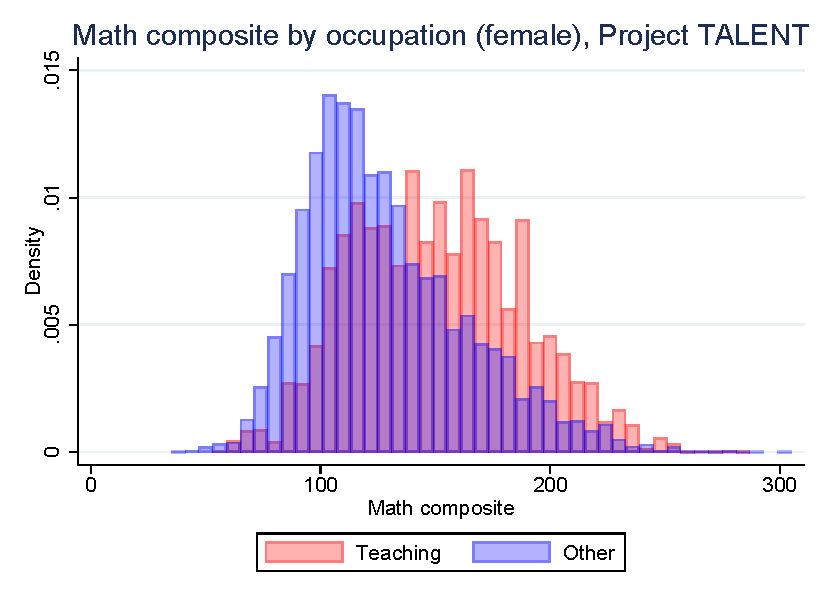
\includegraphics[width=0.5\textwidth]{plots/TALENT_math_occ_no_norm_female_no_lf.pdf}
				% 		\end{figure}
			% 		\vfill
			% 	\end{adjustwidth}
		% \end{frame}
	
	\begin{frame}
		\frametitle{Stylized Fact \#4}
		\framesubtitle{Trends in Ability Distribution of Females by Occupation}
		\begin{adjustwidth}{2em}{2em}
			\vfill
			\begin{figure}[ht!]
				\begin{subfigure}[b]{0.29\textwidth}
					\centering
					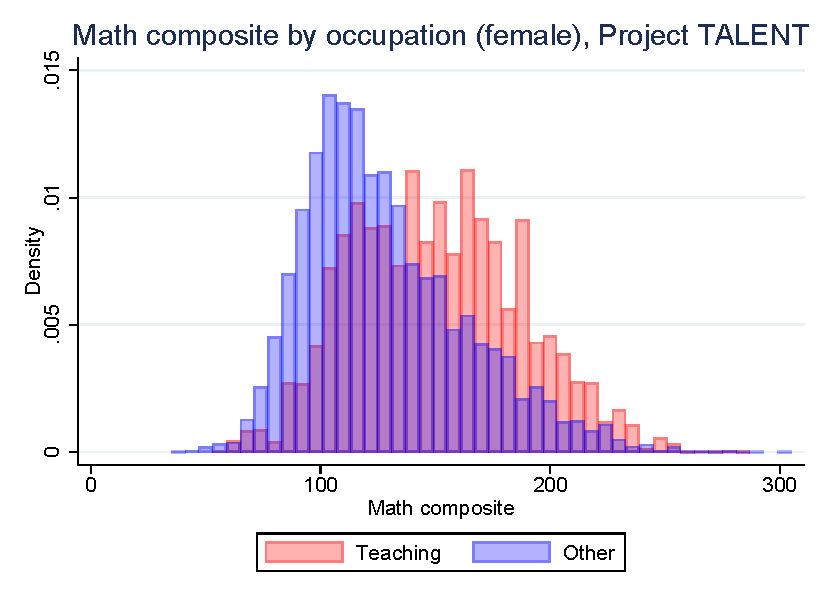
\includegraphics[width=\textwidth]{plots/TALENT_math_occ_no_norm_female_no_lf.pdf}
				\end{subfigure}
				\hfill
				\begin{subfigure}[b]{0.27\textwidth}
					\centering
					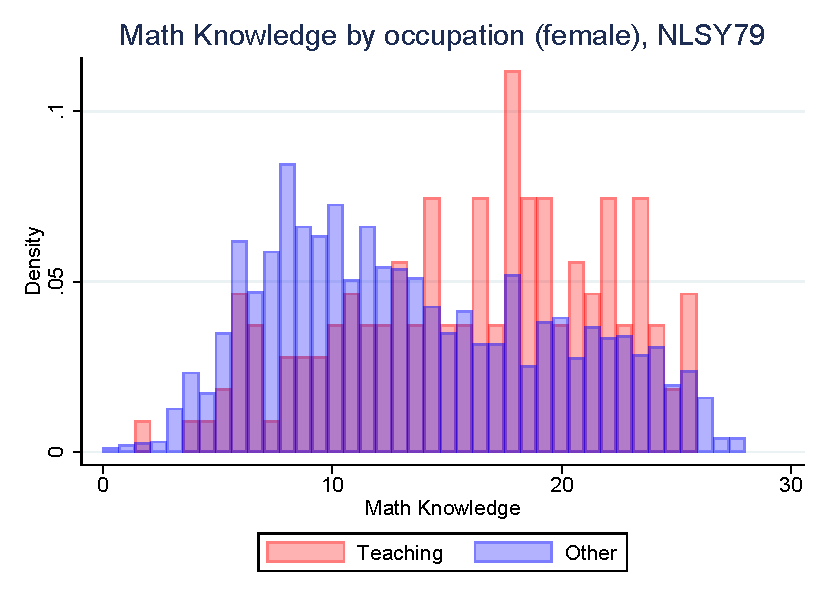
\includegraphics[width=\textwidth]{plots/nlsy79_mk_occ_no_norm_female_no_lf.pdf}
				\end{subfigure}
				\hfill
				\begin{subfigure}[b]{0.27\textwidth}
					\centering
					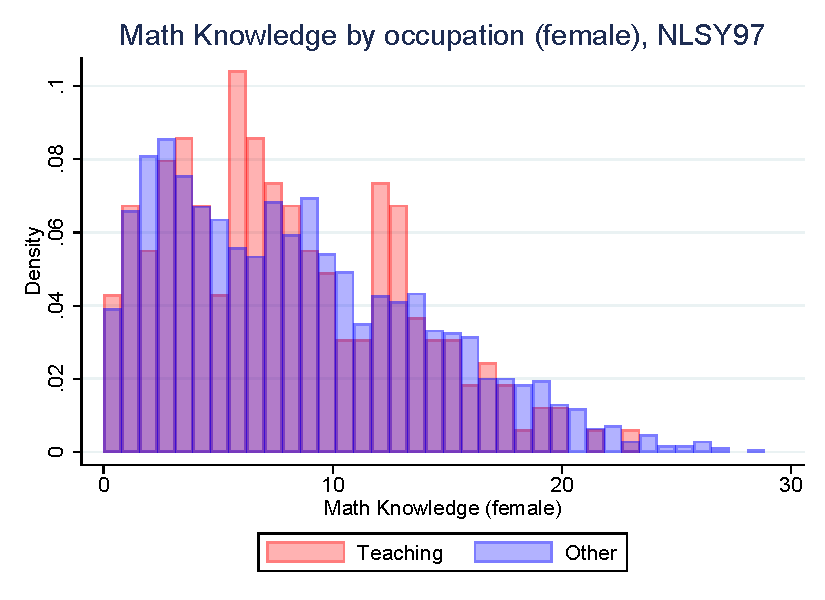
\includegraphics[width=\textwidth]{plots/nlsy97_mk_occ_no_norm_female_no_lf.pdf}
				\end{subfigure}	
				\vfill	
				\begin{subfigure}[b]{0.27\textwidth}
					\centering
					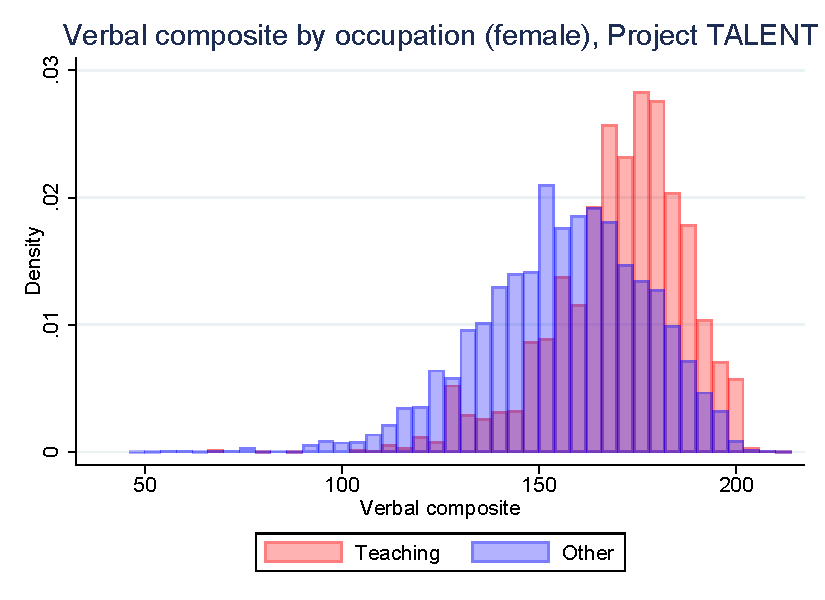
\includegraphics[width=\textwidth]{plots/TALENT_verbal_occ_no_norm_female_no_lf.pdf}
				\end{subfigure}
				\hfill
				\begin{subfigure}[b]{0.27\textwidth}
					\centering
					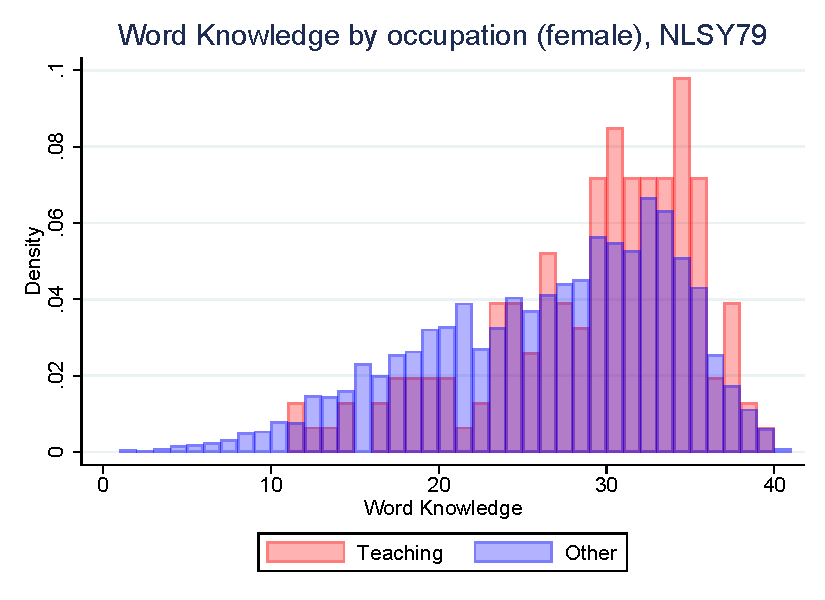
\includegraphics[width=\textwidth]{plots/nlsy79_wk_occ_no_norm_female_no_lf.pdf}
				\end{subfigure}
				\hfill
				\begin{subfigure}[b]{0.27\textwidth}
					\centering
					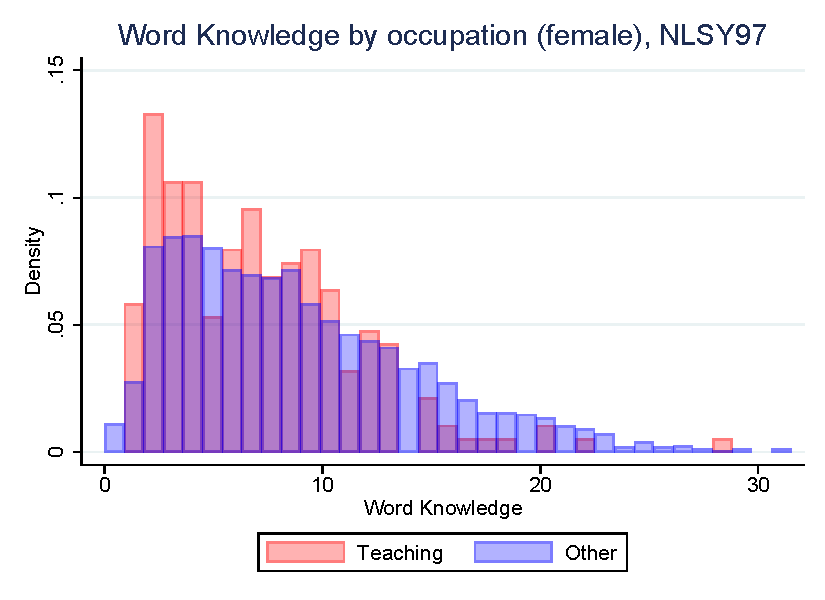
\includegraphics[width=\textwidth]{plots/nlsy97_wk_occ_no_norm_female_no_lf.pdf}
				\end{subfigure}	
			\end{figure}
			\vfill
		\end{adjustwidth}
	\end{frame}
	
	\begin{frame}
		\frametitle{Model}
		\framesubtitle{Three Major Building Blocks}
		\begin{itemize}
			\item OLG
			\item Non-linear version of occupational choice model
			\item Educational barriers / labor market discrimination \\
			(as in Hsieh et al., 2019)
		\end{itemize}
	\end{frame}
	
	\begin{frame}
		\frametitle{Model}
		\framesubtitle{Endowments, Preferences}
		\begin{itemize}
			\item Each period, a measure $M$ of agents is born and lives for two periods: ``young'' and ``old''
			\item $G$ groups of individuals
			\item $I$ occupations indexed by $i \in \{1,\dots,I\}$
			\item Occupational abilities $\vec{a}$ drawn from joint distribution $F(\vec{a})$
			\item $\log$ preferences over consumption and leisure:
			\begin{displaymath}
				\mu \ln C'_{g} + \ln\left(1-s_{i,g} \right)
			\end{displaymath}
		\end{itemize}
	\end{frame}
	
	\begin{frame}
		\frametitle{Simple Two-Sector Model}
		\framesubtitle{Technologies}
		\begin{itemize}
			\item ``Young'' make occupation-specific time and goods investments
			\item ``Old'' work as \alert{teachers} or \alert{production workers}
			%  \item Technologies are occupation-specific:
			\begin{description}
				\item[Human capital production] (teaching) depends on\\
				teacher's $h_{T,\hat{g}}$, class size $N(h_{T,\hat{g}})$,  own ability $a_i$, time $s_{i,g}$ and goods $e_{i,g}$ investments:
				\begin{align*}
					\label{}
					h'_{i,g}(a_i) & =\left( h_{T,\hat{g}}\right)^\beta a_i^\alpha(s_{i,g})^{\phi} (e_{i,g})^{\eta}\big(N(h_{T,\hat{g}})\big)^{-\sigma}\\
					& \textrm{{\sf where }} \widetilde{H}_T =\sum_{\hat{g}=1}^G \int_0^\infty \left( h_{T,\hat{g}}\left( a \right) \right)^{\frac{\beta}{\sigma}} f_{T,\hat{g}}(a) da
				\end{align*}
				\item[Final output production] depends on adult worker's human capital $h_{O,g}$ and exogenous productivity $A_O$:
				\begin{align*}
					\label{}
					y_g = A_O h_{O,g}
				\end{align*}
			\end{description}
		\end{itemize}
	\end{frame}
	
	
	\begin{frame}
		\frametitle{Simple Two-Sector Model}
		\framesubtitle{Values}
		\begin{align*}
			\label{}
			V_g(a_T,a_O,\widetilde{H}_T) & = \max_{\{s_{O,g},s_{T,g},e_{O,g},e_{T,g}\}} \bigg\{ V_{O,g}(a_O,\widetilde{H}_T), V_{T,g}(a_T,\widetilde{H}_T) \bigg\} \label{eq:V}
		\end{align*}
		where
		\begin{align*}
			%\label{eq:vo}
			V_{O,g}(a_O,\widetilde{H}_T) & = \ln\left(1-s_{O,g}\left(a_O,\widetilde{H}_T\right)\right) \nonumber \\
			& + \mu \ln \Big[ {{h'}_{O,g}} A_O'(1-t')\alert{(1-\tau^{\omega '}_{O,g})} \nonumber \\
			& - e_{O,g}(a_O,\widetilde{H}_T)\alert{(1+\tau^e_{O,g})} \Big],\\
			%\label{eq:vt}
			V_{T,g}(a_T,\widetilde{H}_T) & = \ln\left(1-s_{T,g}\left(a_T,\widetilde{H}_T\right)\right) \nonumber \\
			& + \mu \ln \Big[ \omega_{T,g}'({h_{T,g}'})(1-t')\alert{(1-\tau^{\omega '}_{T,g}) }\nonumber \\
			& - e_{T,g}(a_T,\widetilde{H}_T)\alert{(1+\tau^{e }_{T,g})} \Big] 
		\end{align*}
	\end{frame}
	
	\begin{frame}
		\frametitle{Simple Two-Sector Model}
		\framesubtitle{Constraints}
		\begin{align*}
			%H^{T} & = \int_{0}^{\infty} \left(h^{T}(a)\right)^{\frac{\beta}{\sigma}} f^{T}(a) da \\
			\alert{t}\Bigg[ \sum_{g=1}^G \int_0^\infty (1-\tau^{\omega}_{T,g})\omega_{T,g}\left(h_{T,g}(a)\right) f_{T,g}(a) da  \\
			+ \sum_{g=1}^G \int_0^\infty (1-\tau^{\omega}_{O,g})A_O h_{O,g}(a) f_{O,g}(a) da \Bigg]\\
			= \sum_{g=1}^G \int_0^\infty (1-\tau^{\omega}_{T,g})\omega_{T,g}\left(h_{T,g}(a)\right) f_{T,g}(a) da \\
			f_{T,g}(a)  = \int_0^{\bar{a}_g^{-1}\left(a\right)} f\big(a,b \big) db \\
			f_{O,g}(b)  = \int_0^{\bar{a}_g\left(b\right)} f\big(a,b \big) da 
			%f^T(a) & = \int_0^{\bar{a}\big(a;H^T,{H^T}'\big)} f\big(a,a^O\big) da^O 
		\end{align*}		
	\end{frame}
	
	\begin{frame}
		\frametitle{Simple Two-Sector Model}
		\framesubtitle{Laws of Motion}
		\begin{align*}
			{H}_{O}' & = \sum_{g=1}^G \int_0^\infty \left(\tfrac{2 \widetilde{H}_T}{M}\right)^\sigma a^\alpha s_{O,g}\left(a,\widetilde{H}_T\right)^\phi e_{O,g}(a,\widetilde{H}_T)^\eta  f_{O,g}(a) da \\
			\widetilde{H}_{T}' & = \sum_{g=1}^G \int_0^\infty \left(\left(\tfrac{2 \widetilde{H}_T}{M}\right)^\sigma a^\alpha s_{T,g}\left(a,\widetilde{H}_T\right)^\phi e_{T,g}(a,\widetilde{H}_T)^\eta \right)^{\alert{\frac{\beta}{\sigma}}} f_{T,g}(a) da 
		\end{align*}
	\end{frame}
	
	\begin{frame}
		\frametitle{Simple Two-Sector Model}
		\framesubtitle{Occupational Threshold}
		\begin{equation*}
			%\label{eq:ot}
			a^*_{T,g}(a_O) = \bar{a}_g\big(a_{O},\widetilde{H}_T\big) %\\
		\end{equation*}
		such that
		\begin{equation}
			\label{eq:indiff}
			V_{O,g}(a_{O},\widetilde{H}_T) = V_{T,g}\left(a^*_{T,g}(a_O),\widetilde{H}_T\right) \textrm{{\sf , for all} } a_O \in (0,\infty) \nonumber
		\end{equation}
	\end{frame}
	
	\begin{frame}
		\frametitle{Model}
		%\small
		%\begin{description}
		%  \item[Problem \#1:] We don't know $\omega(\cdot,\cdot)$ and we need to compute it numerically!
		%  \item[Challenge:] $\omega(\cdot,\cdot)$ is possibly non-linear in $h^T$ (for given $H^T$) 
		%  \item[Problem \#2:] For given $\omega(\cdot,\cdot)$, need to identify the fixed point $H^{T'} = {\widetilde{H^{T'}}} $.
		%  \item[Solution:] $\omega(\cdot,\cdot)$ is proportional to the \textit{number of students} in a teacher's class:
		%  \begin{equation*}
			%\omega(h^T,H^T) = \lambda N(h^T,H^T) = \lambda \frac{M}{2 H^T} \left( h^T \right)^{\frac{\beta}{\sigma}}
			%\end{equation*}
			\begin{itemize}
				\item Assignment of students to teachers is random \\ $\Rightarrow$ distribution of students' skill identical across classrooms
				\item Teachers with different $h_{T,g}$ vary with respect to class {\it size}
				\begin{align*}
					N(h_{T,g})=h_{T,g}^\frac{\beta}{\sigma} \cdot \frac{M}{2\widetilde{H}_T}
				\end{align*}
				\item Teacher's wage $\omega_{T,g}$ depends on teacher's human capital:
				%\item $\omega(\cdot,\cdot)$ is proportional to the \textit{number of students} in a teacher's class:
				\begin{align*}
					\omega_T(h_{T,g})  =  \kappa h_{T,g}^\gamma 
					%\omega(h_{T,g},\widetilde{H}_T) & =  \lambda N(h^T,\widetilde{H}^T) \\
					%& = \frac{{H'}^O {A'}^O}{\frac{M}{2}\sum_{g=1}^G \int_0^\infty f_{O,g}(a) da} \cdot %\underbrace{\overbrace{N(1,\widetilde{H}^T)}^{=\frac{M}{2}\frac{1}{\widetilde{H}^T}}\left( h^T \right)^{\frac{\beta}{\sigma}}}_{=N(h^T,\widetilde{H}^T)} \\
					%& =\frac{\overbrace{{H}'_O {A}'_O}^{\textrm{total output (next period)}}}{\underbrace{\sum_{g=1}^G \int_0^\infty f_{O,g}(a) da}_{\begin{subarray}{c}\textrm{fraction of prospective} \\ 
					%\textrm{production workers in class}\end{subarray}}} \cdot \underbrace{\frac{\left( h_{T,g} \right)^{\frac{\beta}{\sigma}}}{{\widetilde{H}_T}}}_{\textrm{fraction of students taught}}\\ 
	\end{align*}
	%  \item $\lambda$ is the value of human capital per worker (in units of output) in occupation $O$.
\end{itemize}

%  \item[Implication:] standard Roy model results no longer hold
%\end{description}
\end{frame}

\begin{frame}
\frametitle{Equilibrium}
\label{eqm}
%\small
Given occupational choices of today's ``old'' and aggregate human capital $\widetilde{H}_{T}$ and ${H}_{O}$, the equilibrium consists of individual choices of ``young'' $\{e_{T,g}, s_{T,g}, e_{O,g}, s_{O,g}\}$, the occupational choice boundary $a^*_{T,g}(a_O)$, the corresponding densities $f_{T,g}$ and $f_{O,g}$, and occupation- and group-specific wage profiles $\{\omega_{T,g}, \omega_{O,g}\}$ such that:
\begin{enumerate}
	\item Individuals solve their investment and occupational choice problems \hyperlink{timeinv}{\beamergotobutton{Time Investment}} \hyperlink{goodinv}{\beamergotobutton{Goods Investment}}
	\item Aggregate human capital follows the laws of motion \hyperlink{laws}{\beamergotobutton{Laws of Motion}}
	\item Government budget constraint is satisfied
\end{enumerate}
%\hyperlink{wage}{\beamergotobutton{Wage Profile}} 
%\hyperlink{param}{\beamergotobutton{Parameter Restrictions}}
\end{frame}

%\begin{frame}
%\frametitle{Aggregate laws of motion (cont'd)} 
%There exist a strictly positive, stable fixed point in $\widetilde{H}^T$ if:
%\begin{equation*}
%\beta<1-\eta
%\end{equation*}
%\end{frame}

\begin{frame}
\frametitle{Occupational Choice Boundary\ldots}
\framesubtitle{\ldots depends on aggregate state $\widetilde{H^T}$} 
%\footnotesize
\begin{align*}
	\frac{\alert{\bar{a}_T(a_O)}^\frac{\alpha}{\frac{1}{\gamma}-\eta}}{a_O^\frac{\alpha}{1-\eta}} \cdot \frac{s_{T,g}^\frac{\phi}{\frac{1}{\gamma}-\eta}}{s_{O,g}^\frac{\phi}{1-\eta}}\cdot \frac{\tau_{T,g}^\frac{1}{1-\eta\gamma}}{\tau_{O,g}^\frac{1}{1-\eta}} \cdot \frac{1+\tau^e_{T,g}}{1+\tau^e_{O,g}}\cdot \left(\frac{1-s_{T,g}}{1-s_{O,g}}\right)^\frac{1}{\mu} \nonumber\\
	\times \frac{\left(\kappa \cdot \gamma\right)^\frac{1}{1-\eta\gamma}}{{A'}_O^\frac{1}{1-\eta}} \cdot \frac{\frac{1}{\gamma}-\eta}{1-\eta}\cdot \eta^\frac{\eta(\gamma-1)}{(1-\eta)(1-\eta\gamma)} \cdot \left(\tfrac{2\alert{\widetilde{H}_T}}{M}\right)^{\frac{\sigma(\gamma-1)}{(1-\eta)(1-\eta\gamma)}}=1 \nonumber%\\                
	%\frac{a_O^{\frac{\alpha}{1-\eta}}}{\textcolor{red}{\bar{a}_T(a_O)}^{\frac{\alpha\beta}{\sigma-\eta\beta}}} \cdot \frac{\tau_{O,g}^\frac{1}{1-\eta}}{\tau_{T,g}^\frac{\sigma}{\sigma-\eta\beta}} \cdot \frac{1-\eta}{1-\tfrac{\beta \eta}{\sigma}} \cdot \frac{1+\tau^e_{O,g}}{1+\tau^e_{T,g}} \cdot \left(\frac{1-s_{O,g}}{1-s_{T,g}}\right)^\frac{1}{\mu} \cdot \frac{s_{O,g}^\frac{\phi}{1-\eta}}{s_{T,g}^\frac{\phi\beta}{\sigma-\eta\beta}} \nonumber\\
	%= \frac{\sum_{g=1}^G \tau_{O,g}^\frac{\eta}{1-\eta} \cdot s_{O,g}^{\frac{\phi}{1-\eta}} \cdot \int_0^\infty a^{\frac{\alpha}{1-\eta}} \textcolor{red}{f_{O,g}(a)}da }{\sum_{g=1}^G \tau_{T,g}^\frac{\eta\beta}{\sigma-\eta\beta} \cdot s_{T,g}^\frac{\phi\beta}{\sigma-\eta\beta} \cdot \int_0^\infty a^{\frac{\alpha\beta}{\sigma-\eta\beta}} \textcolor{red}{f_{T,g}(a)}da \cdot \sum_{g=1}^G \int_0^\infty \textcolor{red}{f_{O,g}(a)}da  } \nonumber
\end{align*}
where
\begin{align}
	\tau_{i,g} =\frac{(1-t)(1-\tau^{\omega}_{i,g})}{1+\tau^e_{i,g}} \nonumber
\end{align}
\end{frame}

\begin{frame}
\frametitle{Data}
%\framesubtitle{}
\begin{itemize}
	\item Micro-data on abilities and occupational choice:
	\begin{enumerate}
		\item Project TALENT (1960-1975):
		\begin{itemize}
			\item representative 5\% sample of high school population in 1960
			\item follow-up surveys at 1, 5, and 11-year post graduation
		\end{itemize}
		\item NLSY 79
		\item NLSY 97
	\end{enumerate}
	\item \textit{Math}, \textit{Verbal}, and \textit{Social} abilities
	\item Occupational choice 11 years after (likely) high school graduation in all surveys ($\sim$ age 29)
\end{itemize}
\end{frame}

\begin{frame}
\frametitle{Occupation-specific Abilities}
%\framesubtitle{}
\begin{itemize}
	\item Ability rank from NLSY 79 and NLSY 97: \\
	\textit{Math}, \textit{Verbal}, and \textit{Social} (Guvenen et al, 2020)
	\item ``Crosswalk'' from composite math and verbal scores in Project TALENT to AFQT equivalents (Air Force, 1990)
	\item Social composite in Project TALENT (Deming, 2017)
	\item Skill requirements by occupation from O*NET: \\
	\textit{Math}, \textit{Verbal}, and \textit{Social} (Guvenen et al, 2020)
	\item Occupation-specific ability:
	\begin{align*}
		\bar{a}=\frac{a_m+a_v+a_s}{b_m+b_v+b_s}+\sum_{i=\{m,v,s\}}\frac{a_i}{b_i}\cdot\left|\frac{a_i}{a_v+a_m+a_s}-\frac{b_i}{b_v+b_m+b_s}\right|\nonumber
	\end{align*}  
\end{itemize}
\end{frame}

% \begin{frame}
% \frametitle{Occupational Skills from Cognitive Scores}
% %\framesubtitle{}
% \begin{itemize}
	%   \item Harmonized cognitive scores from NLSY79 and NLSY97 for:
	%   \begin{enumerate}
		%   \item Mathematics knowledge
		%   \item Arithmetic reasoning
		%   \item Word knowledge
		%   \item Paragraph comprehension
		% \end{enumerate}
	%   \item ``Crosswalk'' from composite math and verbal scores in Project TALENT to AFQT equivalents (Air Force)
	%   \item Skill requirements by occupation from O*NET
	%   \item Occupation-specific skills based on ``translation'' of cognitive scores \alert{(work in progress)}
	%   \item In contrast to standard Roy model, occupational choice depends on {\it comparative} \alert{and} {\it absolute} advantage here!
	% \end{itemize}
% \end{frame}

\begin{frame}
\frametitle{Calibration}
\framesubtitle{Assumptions and Normalizations}
\tiny
%			\begin{itemize}
	%  \item $o \in \{1,\ldots,O\}$: index for non-teaching occupations 
	%  \item $T$: index for teaching
	%\end{itemize}
	
	\begin{table}[h!]
		\centering
		\begin{tabular}{lccc}
			\toprule
			\toprule
			Parameter & Definition & Determination & Value\\
			\midrule
			$\tau^{w}_{o,{\rm men}}$ & labor market barriers for men & assumption & 0 \\
			$\tau^{e}_{o,g}$ & human capital barriers for all groups & assumption & 0 \\
			$\tau^{w}_{T,g}$ & labor market barriers in teaching  & assumption & 0 \\
			& (all groups)& &\\
			$\tau^{e}_{T,g}$ & human capital barriers in teaching & assumption & 0 \\
			& (all groups) & &\\
			$\alpha$ & elasticity of human capital with respect to & normalization & 1 \\
			& idiosyncratic ability & &\\
			$\sigma$ & elasticity of human capital with respect to & normalization & 1 \\
			& class size & &\\
			%					$\tau^{e}_{i,g}$ & Human capital barriers for other groups & Normalization & 0 \\
			%					$A_{T}$ & Teachers productivity & Normalization & 1 \\
			%					$\mu_a$ & Mean ability distribution & Normalization & 0 \\
			%					$\sigma_a$ & St.dev. ability distribution & Normalization & 1 \\
			\bottomrule
			%			\bottomrule
		\end{tabular}
		%\caption{Assumptions and Normalization}
		\label{tab:assump}
	\end{table}
\end{frame}

\begin{frame}
	\frametitle{Calibration}
	\framesubtitle{Baseline Parameters}
	\tiny
	\begin{table}[h!]
		\centering
		\begin{tabular}{lccc}
			\toprule
			%					\toprule
			Parameter & Definition & Determination & Value\\
			\midrule
			$\theta$ & shape parameter of Fr\'echet-distributed & wage dispersion in non-teaching occupations & 1.476\\
			& idiosyncratic abilities & (indirect inference) &\\
			%					\midrule
			$\eta$ & goods elasticity of human capital & aggregate education spending share  & 0.103\\
			& & (indirect inference) &\\
			%					\midrule
			$\phi$ & time elasticity of human capital & Mincer returns to education (non-teaching) & 0.999\\
			& & (indirect inference) &\\
			%					\midrule
			$\gamma$ & curvature of wage function in teaching & wage dispersion in teaching & 0.83\\
			&& (indirect inference) &\\
			\midrule
			$\beta$ & elasticity of human capital with respect to & skill composition by occupation and group & 0.5\\
			& teacher's human capital & &\\
			$\mu$ &  trade-off between consumption and & schooling of teachers relative & 0.714\\
			& time spent accumulating human capital & to schooling of others & \\
			\bottomrule
			%			\bottomrule
		\end{tabular}
		%\caption{Baseline Parameter Values}
		\label{tab:param}
	\end{table}
\end{frame}

\begin{frame}
	\frametitle{Calibration}
	\framesubtitle{Baseline Parameters by Year}
	\tiny
	\begin{table}[h!]
		\centering
		\begin{tabular}{lcc}
			\toprule
			%					\toprule
			Parameter & Definition & Determination \\
			\midrule			
			$A_{o}$ & occupational productivities (non-teaching) & labor market shares for men  \\
			%					\midrule
			$\tau^{w}_{o,{\rm women}}$ & labor market barriers (non-teaching) & labor market shares for women \\
			& faced by women & \\
			%					\midrule
			$\kappa$ & scale parameter of wage function in teaching & fraction of males who are teachers \\
			%					\midrule
			$\lambda_f$ & aggregate labor market barrier for women & fraction of females who are teachers \\
			& in non-teaching occupations & \\
			% s_T/s_O, where  s_i=years of school/25 years
			\bottomrule
			%			\bottomrule
		\end{tabular}
		%\caption{Baseline Parameter Values}
		\label{tab:param}
	\end{table}
\end{frame}

% \begin{frame}
	% \frametitle{Calibration}
	% \framesubtitle{$\frac{\beta}{\sigma}$}
	
	% \end{frame}



% \begin{frame}
	% 	\frametitle{Teacher's Wage Profile} 
	% 	\label{wage}
	% 	%The F.O.C.s for $s^T$ and $e^T$, respectively, after a few steps of algebra are:
	% 	\begin{align}
		% 		\omega & = \eta^{\frac{\eta}{1-\eta}}\cdot \left(\tfrac{2\widetilde{H}_T}{M}\right)^{\frac{\sigma}{1-\eta}} \cdot \frac{\sum_{g=1}^G {A_O'}^\frac{1}{1-\eta}\cdot\tau_{O,g}^\frac{\eta}{1-\eta} \cdot s_{O,g}^\frac{\phi}{1-\eta}\cdot \int_0^\infty a^{\frac{\alpha}{1-\eta}} f_{O,g}(a)da}{\sum_{g=1}^G f_{O,g}(a)da} \nonumber\\
		% 		& \times \frac{\tau_{T,g}^\frac{\eta\beta}{\sigma-\eta\beta } \cdot s_{T,g}^\frac{\phi\beta }{\sigma-\eta\beta } \cdot a_T^\frac{\alpha\beta }{\sigma-\eta\beta}}{\sum_{g=1}^G \tau_{T,g}^\frac{\eta\beta }{\sigma-\eta\beta } \cdot s_{T,g}^\frac{\phi\beta }{\sigma-\eta\beta } \cdot \int_0^\infty a^\frac{\alpha\beta}{\sigma-\eta\beta } f^{g,T}(a)da} \nonumber
		% 	\end{align}
	% 	\hyperlink{eqm}{\beamergotobutton{Back}}
	% \end{frame}

% \begin{frame}
	% 	\frametitle{Some Parameter Restrictions}
	% 	\label{param}
	% 	\begin{itemize}
		% 		\item $\beta < 1-\eta$ to guarantee existence of stable $\widetilde{H^T} = \widetilde{H^T}' > 0$
		% 		\item $\tfrac{\sigma}{\beta} > \eta$ and $\mu \phi > 0$ for $s^{T*} \in (0,1)$
		% 		\item $1 > \eta$ and $\mu \phi > 0$ for $s^{O*} \in (0,1)$
		% 	\end{itemize}
	% 	\hyperlink{eqm}{\beamergotobutton{Back}}
	% \end{frame}

%\begin{frame}
%\frametitle{Conclusion}
%
%\end{frame}
%\begin{frame}
%\frametitle{Occupational Threshold}
%\framesubtitle{Variation in Strength of Superstar Effect in Teaching: $\frac{\beta}{\sigma}$}
%\begin{figure}
%\begin{center}
%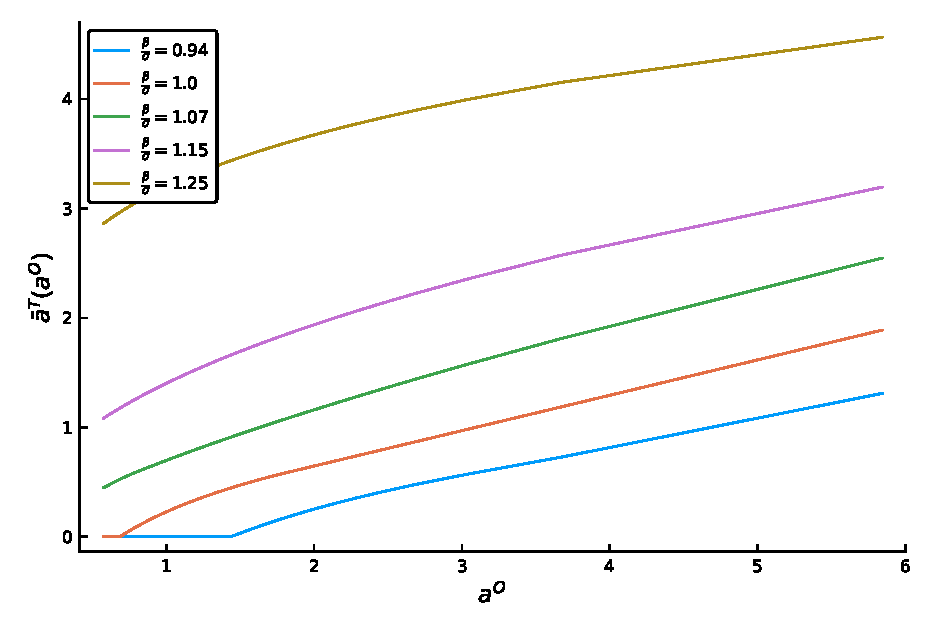
\includegraphics[width=.9\textwidth]{/Users/simeonalder/Dropbox/Work/Research/GitHub/teachers/julia/plots/occ_thresh_tauW_0.0_tauE_0.0_A=2.0.eps}
%%\caption{ }
%%\label{ }
%\end{center}
%\end{figure}
%\end{frame}
%
%\begin{frame}
%\frametitle{Occupational Choice (Aggregate)}
%\framesubtitle{Variation in Strength of Superstar Effect in Teaching: $\frac{\beta}{\sigma}$}
%\begin{figure}
%\begin{center}
%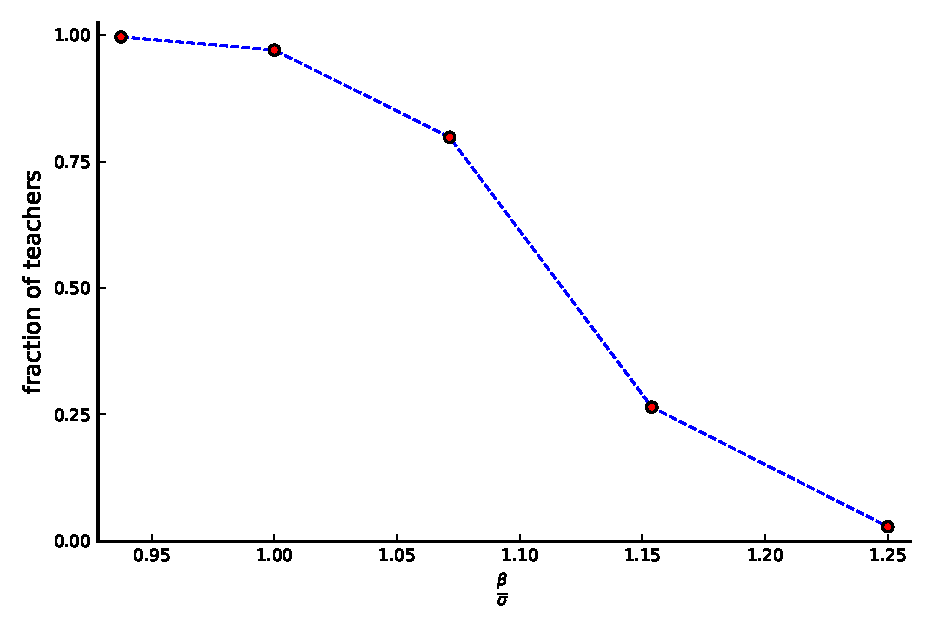
\includegraphics[width=.9\textwidth]{/Users/simeonalder/Dropbox/Work/Research/GitHub/teachers/julia/plots/frac_teachers_tauW_0.0_tauE_0.0_A=2.0.eps}
%%\caption{ }
%%\label{ }
%\end{center}
%\end{figure}
%\end{frame}
%
%\begin{frame}
%\frametitle{Occupational Split}
%\framesubtitle{Variation in Strength of Superstar Effect in Teaching: $\frac{\beta}{\sigma}$}
%\begin{figure}
%\begin{center}
%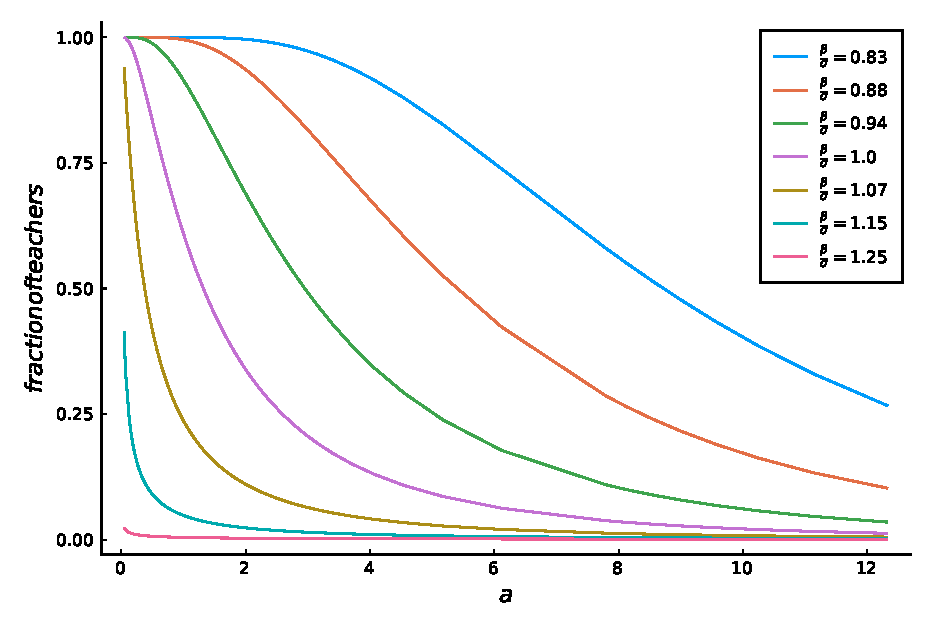
\includegraphics[width=.9\textwidth]{/Users/simeonalder/Dropbox/Work/Research/GitHub/teachers/julia/plots/frac_teachers_by_a_tauW_0.0_tauE_0.0_A=2.0.eps}
%%\caption{ }
%%\label{ }
%\end{center}
%\end{figure}
%\end{frame}
%
%\begin{frame}
%\frametitle{Aggregate Law of Motion for $\widetilde{H^T}$}
%\framesubtitle{Variation in Strength of Superstar Effect in Teaching: $\frac{\beta}{\sigma}$}
%\begin{figure}
%\begin{center}
%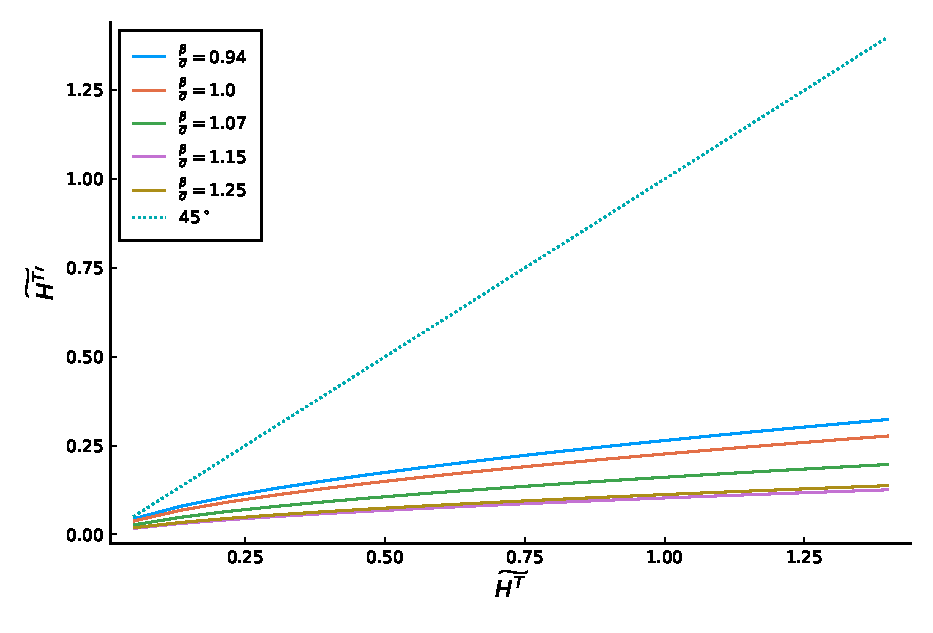
\includegraphics[width=.9\textwidth]{/Users/simeonalder/Dropbox/Work/Research/GitHub/teachers/julia/plots/law_of_motion_tauW_0.0_tauE_0.0_A=2.0.eps}
%%\caption{ }
%%\label{ }
%\end{center}
%\end{figure}
%\end{frame}
%
%\begin{frame}
%\frametitle{Effect of $\tau^w$ on Occupational Choice}
%\framesubtitle{$\frac{\beta}{\sigma} = 1.15$}
%\begin{figure}
%\begin{center}
%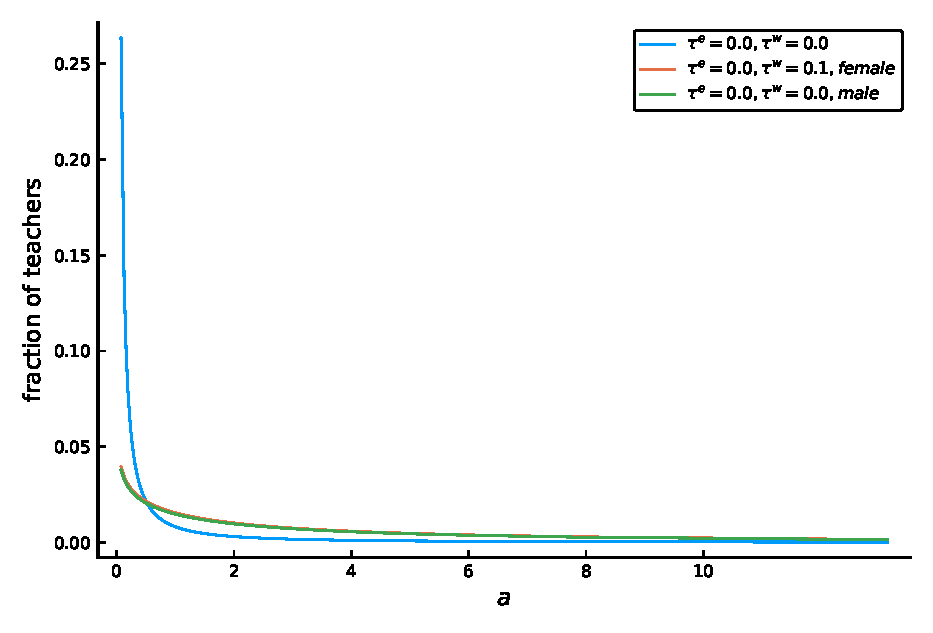
\includegraphics[width=.9\textwidth]{/Users/simeonalder/Dropbox/Work/Research/GitHub/teachers/julia/plots/frac_teachers_by_a_tauW_0.1_tauE_0.0_A=2.0.eps}
%%\caption{ }
%%\label{ }
%\end{center}
%\end{figure}
%\end{frame}
%
%\begin{frame}
%\frametitle{Effect of $\tau^e$ on Occupational Choice}
%\framesubtitle{$\frac{\beta}{\sigma} = 1.15$}
%\begin{figure}
%\begin{center}
%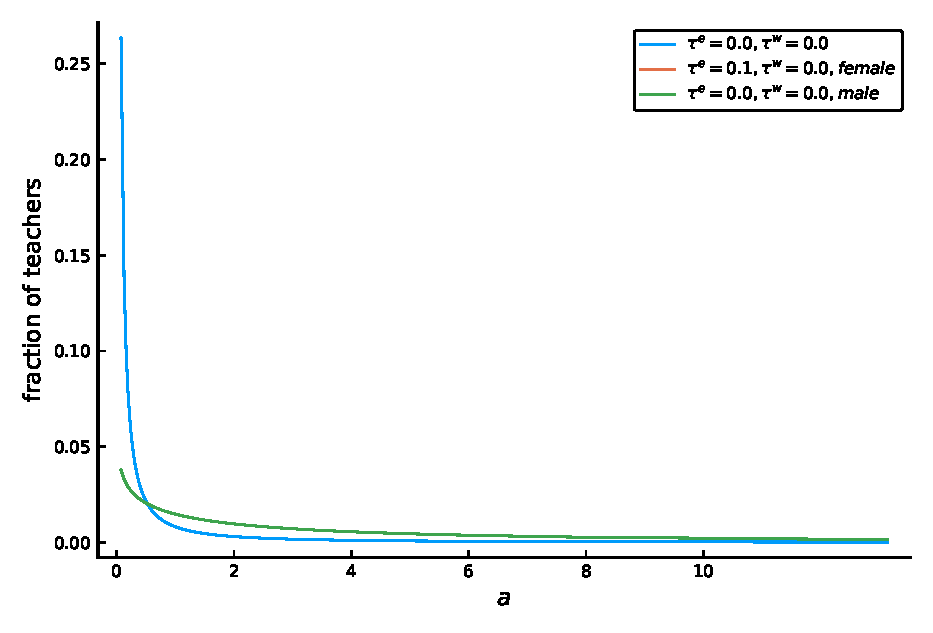
\includegraphics[width=.9\textwidth]{/Users/simeonalder/Dropbox/Work/Research/GitHub/teachers/julia/plots/frac_teachers_by_a_tauW_0.0_tauE_0.1_A=2.0.eps}
%%\caption{ }
%%\label{ }
%\end{center}
%\end{figure}
%\end{frame}
%
%\begin{frame}
%\frametitle{Combined Effect of $\tau^w$ and $\tau^e$ on Occupational Choice}
%\framesubtitle{$\frac{\beta}{\sigma} = 1.15$}
%\begin{figure}
%\begin{center}
%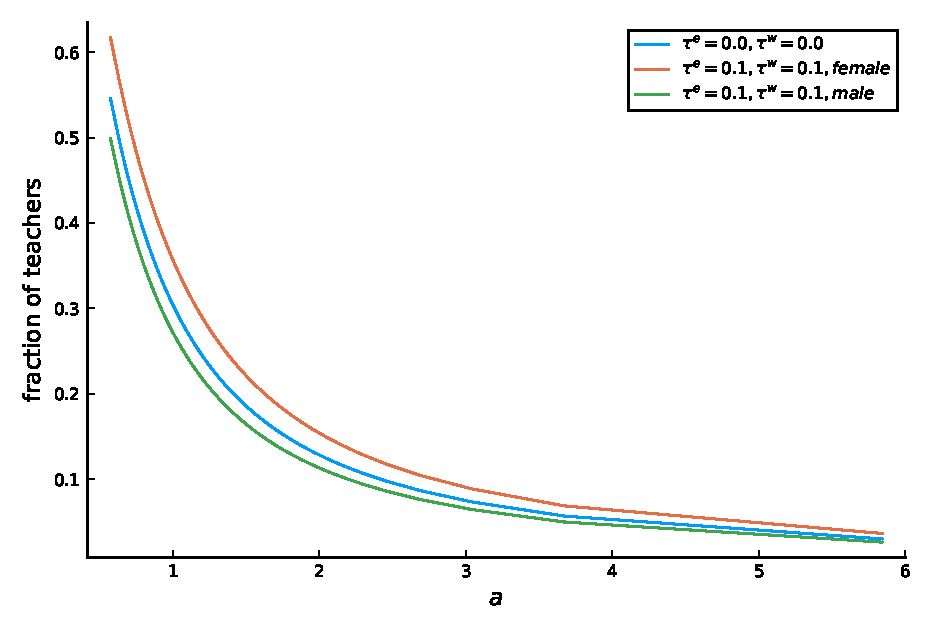
\includegraphics[width=.9\textwidth]{/Users/simeonalder/Dropbox/Work/Research/GitHub/teachers/julia/plots/frac_teachers_by_a_tauW_0.1_tauE_0.1_A=2.0.eps}
%%\caption{ }
%%\label{ }
%\end{center}
%\end{figure}
%\end{frame}

%\begin{frame}
%\frametitle{Extensions}
%\begin{itemize}
%  \item Multiple locations:
%  \begin{itemize}
	%  \item finite number of locations
	%  \item teachers' salaries funded by combination of local lump-sum (property) and proportional (sales) taxes
	%  \item one location with $T=0$, all locations have $t \in (0,1)$
	%  \item sorting of teachers and children into locations (high wage = high tax)
	%  \item sorting breaks global monotonicity between teacher's $h^T$ and class size (still holds locally, with random within-district assignment)
	%  \item to start with, solve with two locations (``high vs.~low'') 
	%  \end{itemize}
%\end{itemize}
%\end{frame}

% CHANGE IN BARRIERS
\begin{frame}
	\frametitle{Labor Market Barriers}
	\label{barriers}
	\begin{figure}
		\begin{center}
			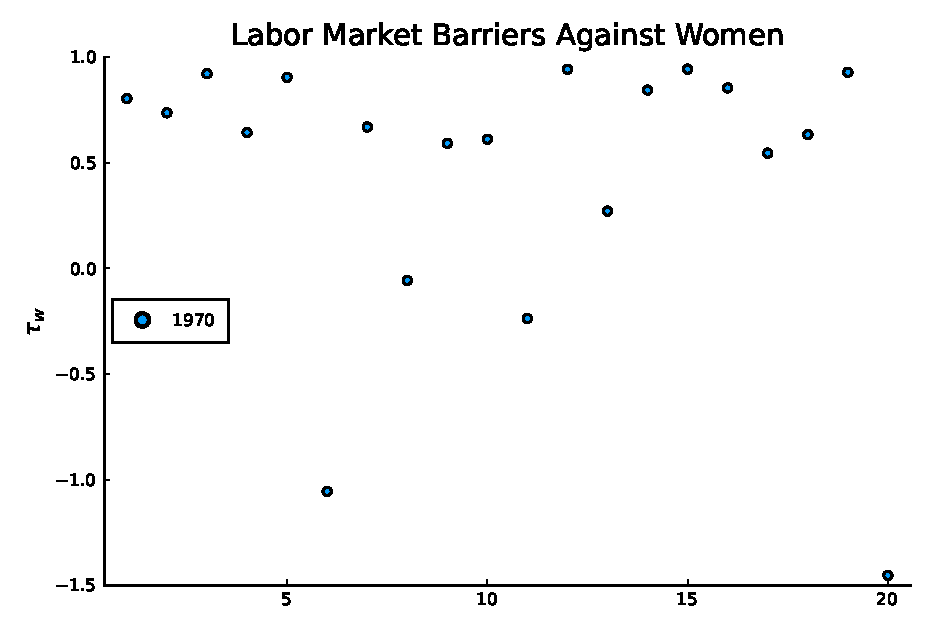
\includegraphics[width=0.8\textwidth]{plots/tau_w_women_70.eps}
			%\caption{ }
			\label{ }
		\end{center}
	\end{figure}
	\hyperlink{occupations}{\beamergotobutton{Occupations}}
\end{frame}

\begin{frame}
	\frametitle{Labor Market Barriers}
	\begin{figure}
		\begin{center}
			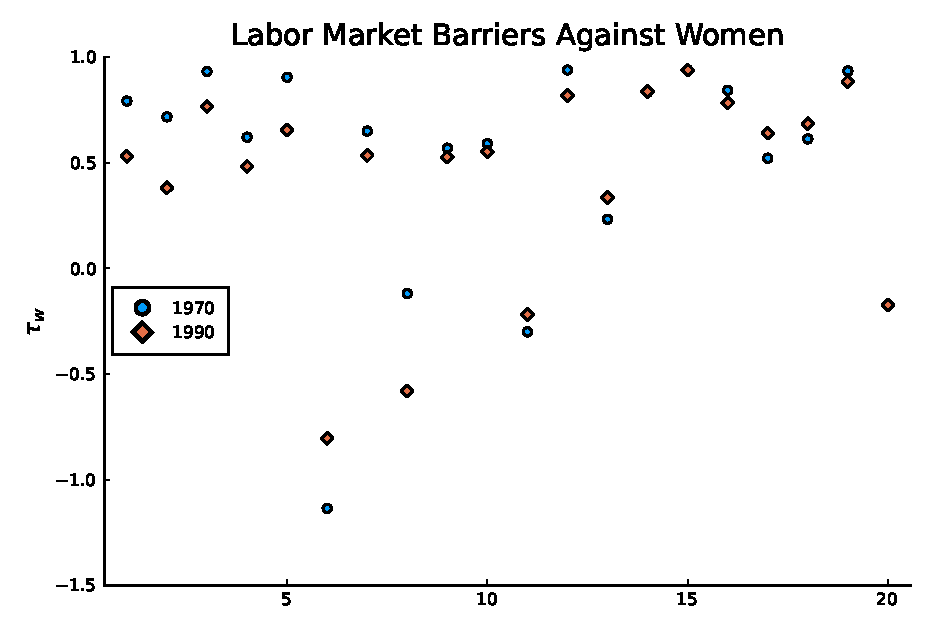
\includegraphics[width=0.8\textwidth]{plots/tau_w_women_70_90.eps}
			%\caption{ }
			\label{ }
		\end{center}
	\end{figure}
	\hyperlink{occupations}{\beamergotobutton{Occupations}}
\end{frame}

\begin{frame}
	\frametitle{Labor Market Barriers}
	\label{barriers3}
	\begin{figure}
		\begin{center}
			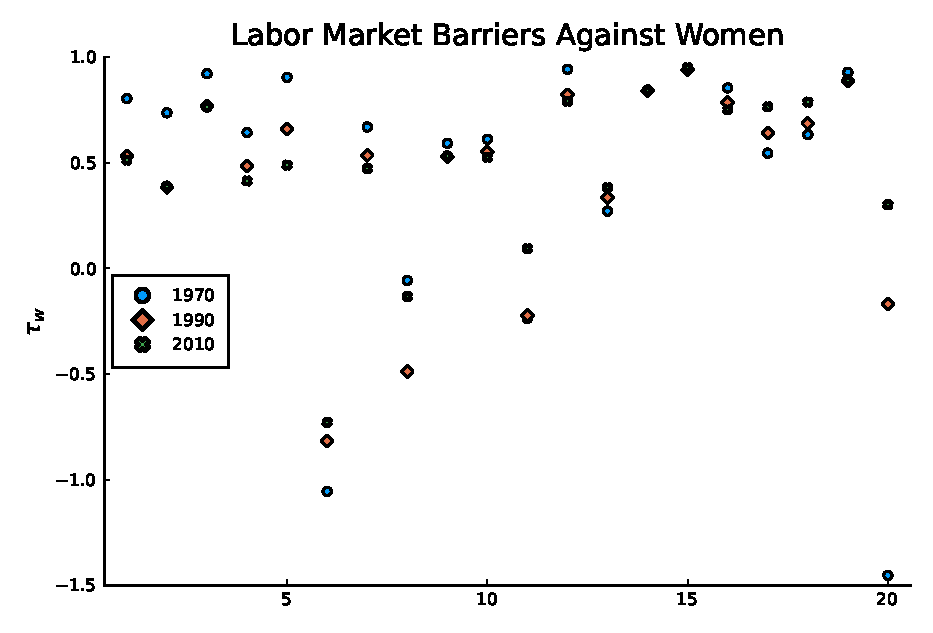
\includegraphics[width=0.8\textwidth]{plots/tau_w_women_70_10.eps}
			%\caption{ }
			\label{ }
		\end{center}
	\end{figure}
	\hyperlink{occupations}{\beamergotobutton{Occupations}}
	\hyperlink{aggprod}{\beamergotobutton{Occupational Productivity}}
\end{frame}

\begin{frame}
	\frametitle{Distribution of Teaching Abilities}
	\framesubtitle{Female workers with lower abilities become teachers}
	\begin{figure}
		\begin{center}
			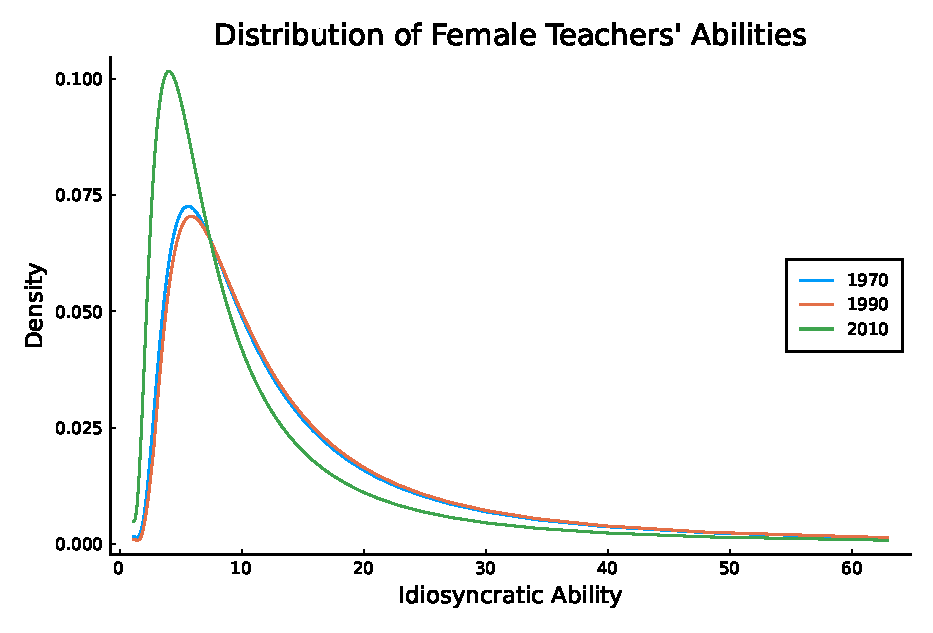
\includegraphics[width=0.8\textwidth]{plots/fT_women_steadystate.eps}
			\label{ }
		\end{center}
	\end{figure}
\end{frame}

\begin{frame}
	\frametitle{Distribution of Teaching Abilities}
	\framesubtitle{Male workers with higher abilities become teachers}
	\begin{figure}
		\begin{center}
			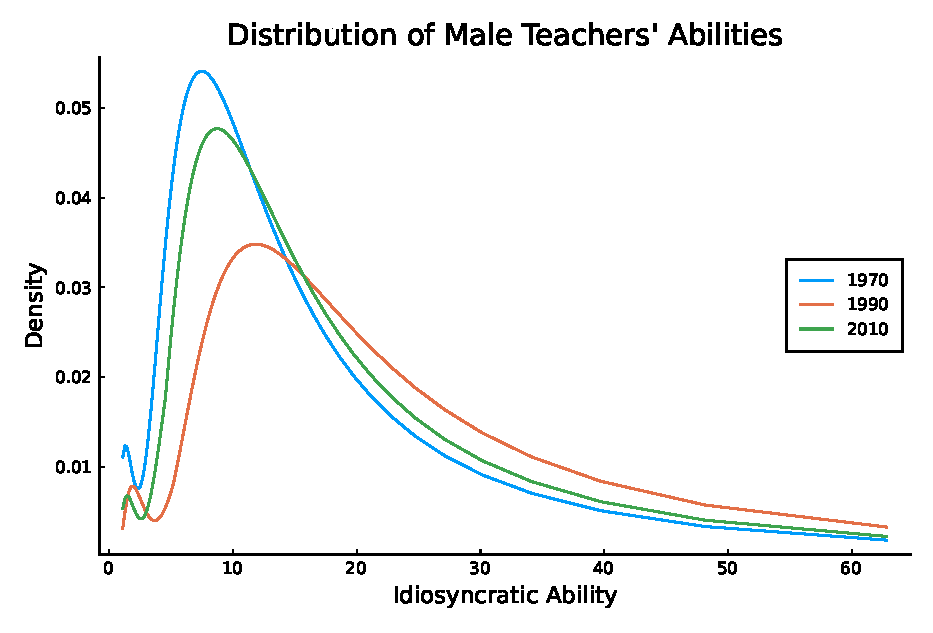
\includegraphics[width=0.8\textwidth]{plots/fT_men_steadystate.eps}
			\label{ }
		\end{center}
	\end{figure}
\end{frame}

%\begin{frame}
%\begin{figure}
%\begin{center}
%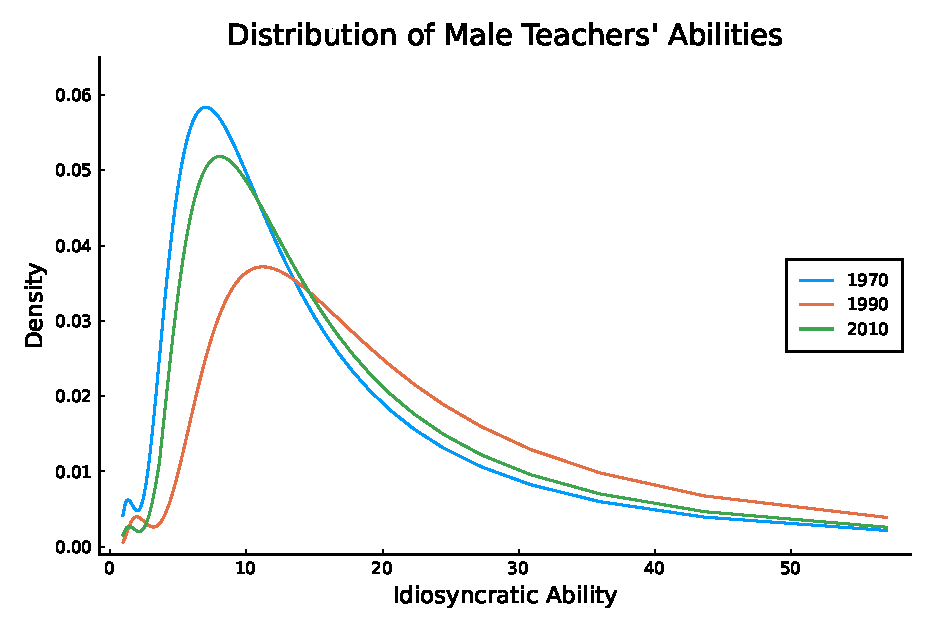
\includegraphics[width=\textwidth]{fT_men_steadystate.eps}
%\caption{ }
%\label{ }
%\end{center}
%\end{figure}
%\end{frame}

\begin{frame}
	\frametitle{Human Capital Investment}
	\framesubtitle{Human capital investment decline over time, given ability}
	\begin{figure}
		\begin{center}
			\includegraphics[width=0.8\textwidth]{plots/eT_women_steadystate.eps}
			%\caption{ }
			\label{ }
		\end{center}
	\end{figure}
\end{frame}


% \begin{frame}
	% \frametitle{Distribution of Teaching Human Capital}
	% \framesubtitle{Female teachers have lower human capital}
	% \begin{figure}
		% \begin{center}
			% \begin{subfigure}[b]{0.49\textwidth}
				% \centering
				% 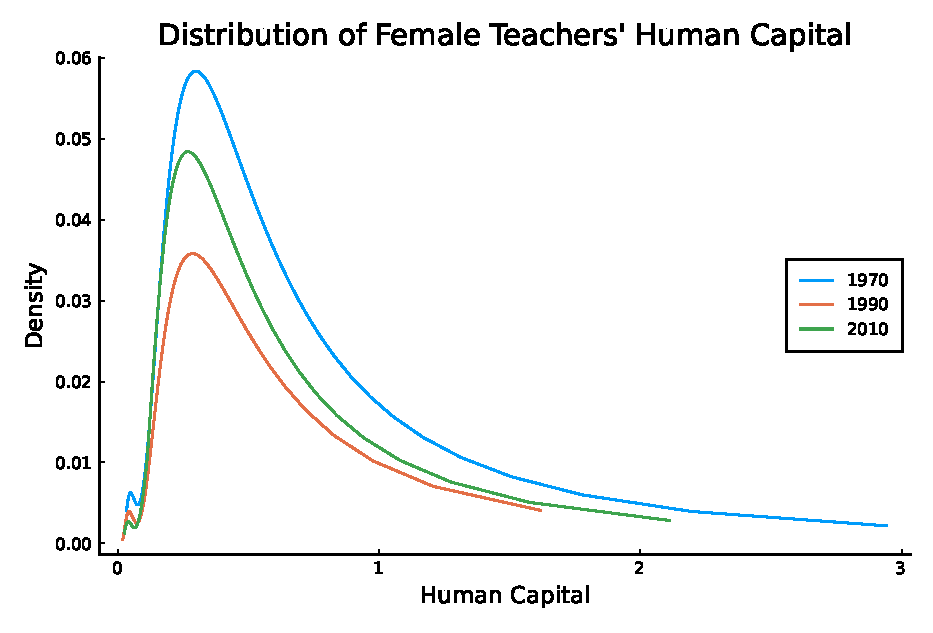
\includegraphics[width=\textwidth]{hT_fT_women_steadystate.eps}
				% \end{subfigure}
			% \hfill
			% \begin{subfigure}[b]{0.49\textwidth}
				% \centering
				% 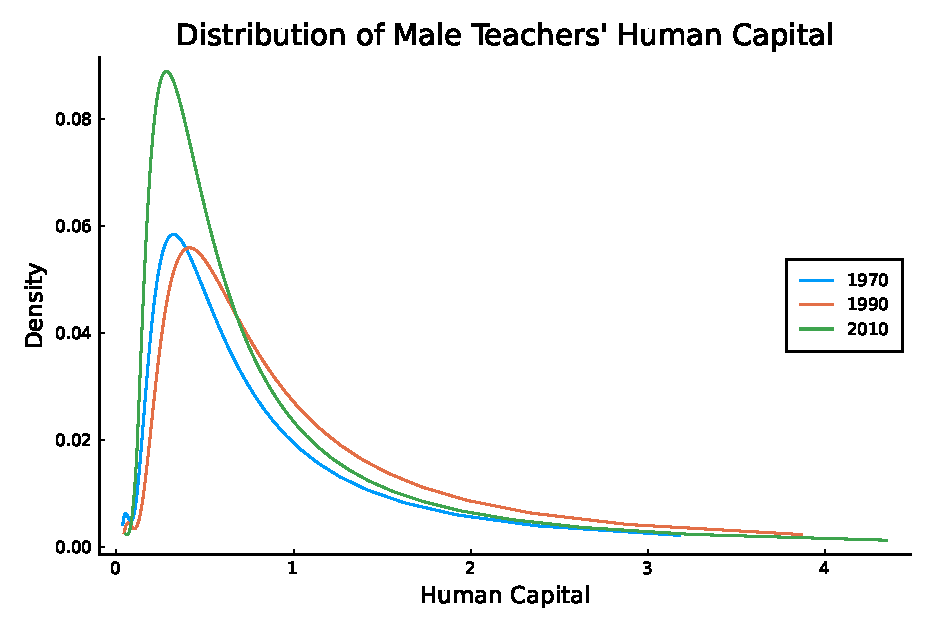
\includegraphics[width=\textwidth]{hT_fT_men_steadystate.eps}
				% \end{subfigure}
			
			%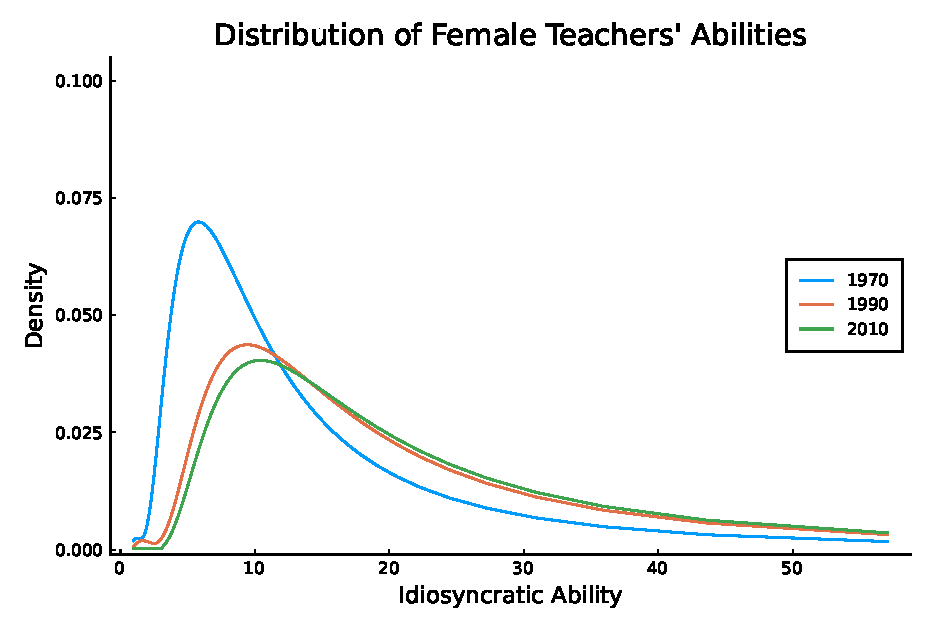
\includegraphics[width=\textwidth]{fT_women_steadystate.eps}
			%\caption{ }
			% \label{ }
			% \end{center}
		% \end{figure}
	% \end{frame}

% \begin{frame}
	% \frametitle{Distribution of Teaching Human Capital}
	% \framesubtitle{}
	% \begin{figure}
		%  		\begin{center}
			%  			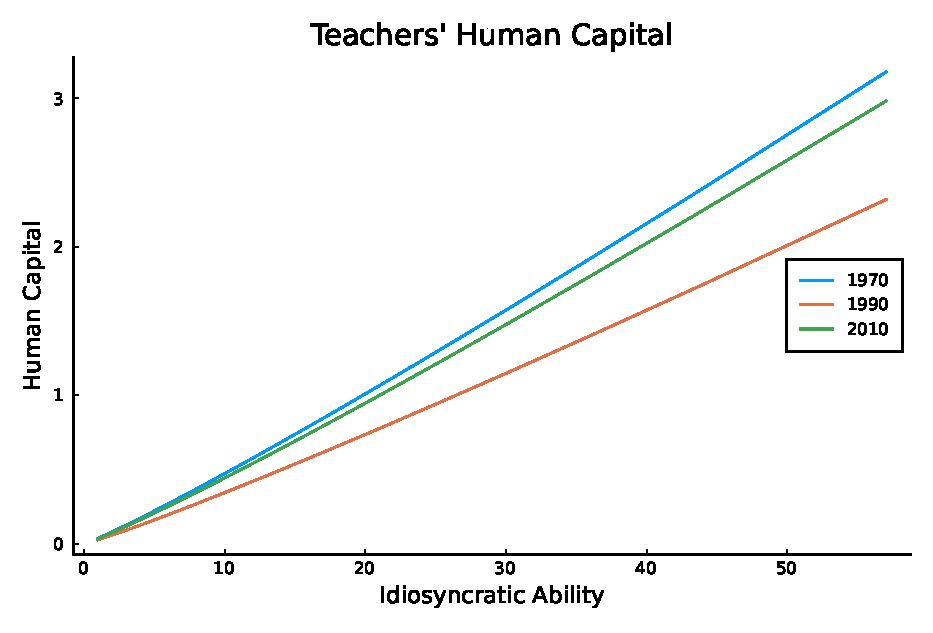
\includegraphics[width=0.8\textwidth]{hT_women_steadystate.eps}
			%  			%\caption{ }
			%  			\label{ }
			%  		\end{center}
		%  	\end{figure}
	% \end{frame}


% \begin{frame}
	% 	\begin{figure}
		% 		\begin{center}
			% 			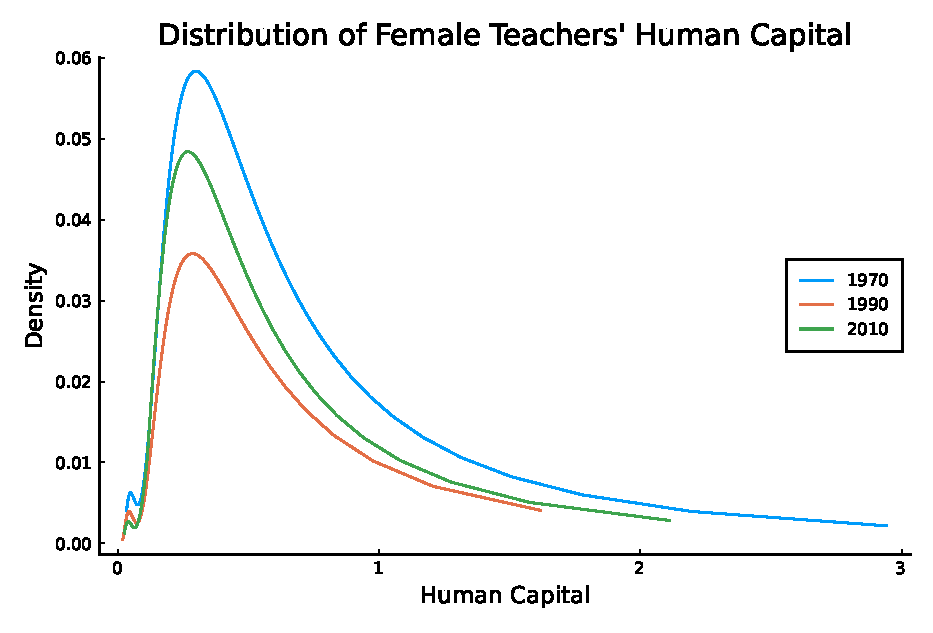
\includegraphics[width=\textwidth]{hT_fT_women_steadystate.eps}
			% 			%\caption{ }
			% 			\label{ }
			% 		\end{center}
		% 	\end{figure}
	% \end{frame}

% \begin{frame}
	% 	\begin{figure}
		% 		\begin{center}
			% 			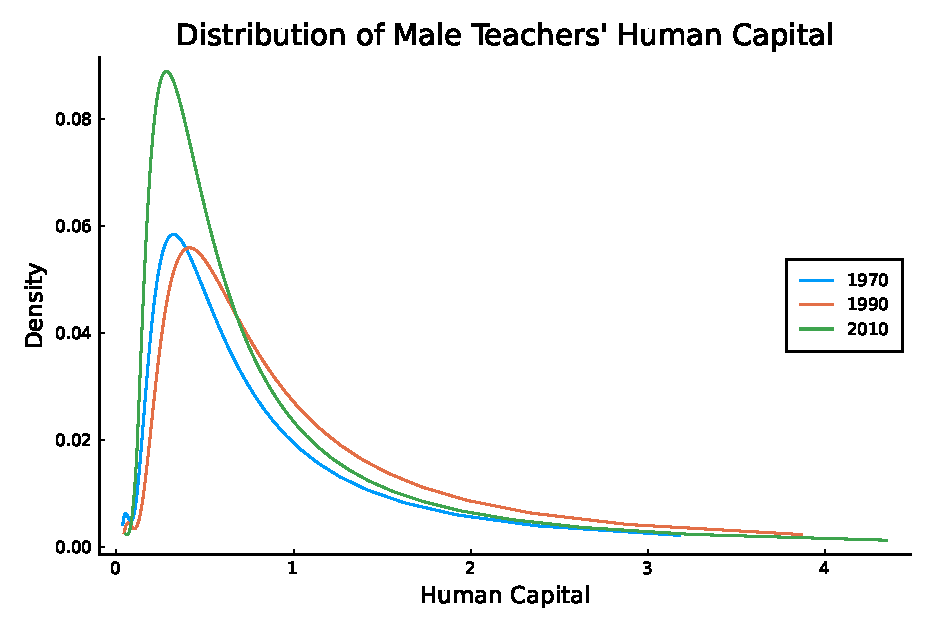
\includegraphics[width=\textwidth]{hT_fT_men_steadystate.eps}
			% 			%\caption{ }
			% 			\label{ }
			% 		\end{center}
		% 	\end{figure}
	% \end{frame}

% \begin{frame}
	% 	\begin{figure}
		% 		\begin{center}
			% 			\includegraphics[width=\textwidth]{eT_women_steadystate.eps}
			% 			%\caption{ }
			% 			\label{ }
			% 		\end{center}
		% 	\end{figure}
	% \end{frame}

% \begin{frame}
	% 	\begin{figure}
		% 		\begin{center}
			% 			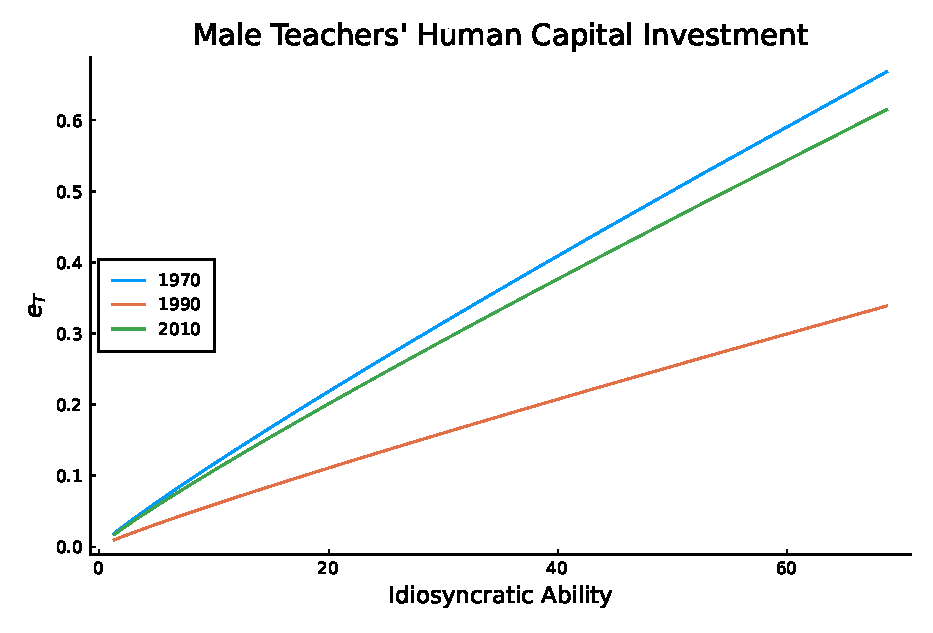
\includegraphics[width=\textwidth]{eT_men_steadystate.eps}
			% 			%\caption{ }
			% 			\label{ }
			% 		\end{center}
		% 	\end{figure}
	% \end{frame}

% \begin{frame}
	% 	\begin{figure}
		% 		\begin{center}
			% 			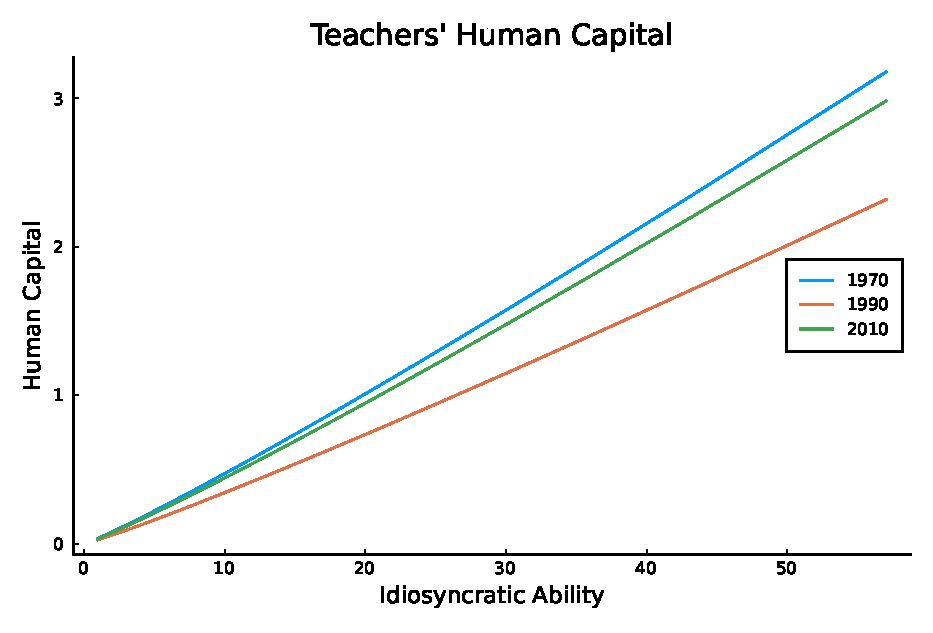
\includegraphics[width=\textwidth]{hT_women_steadystate.eps}
			% 			%\caption{ }
			% 			\label{ }
			% 		\end{center}
		% 	\end{figure}
	% \end{frame}

% \begin{frame}
	% 	\begin{figure}
		% 		\begin{center}
			% 			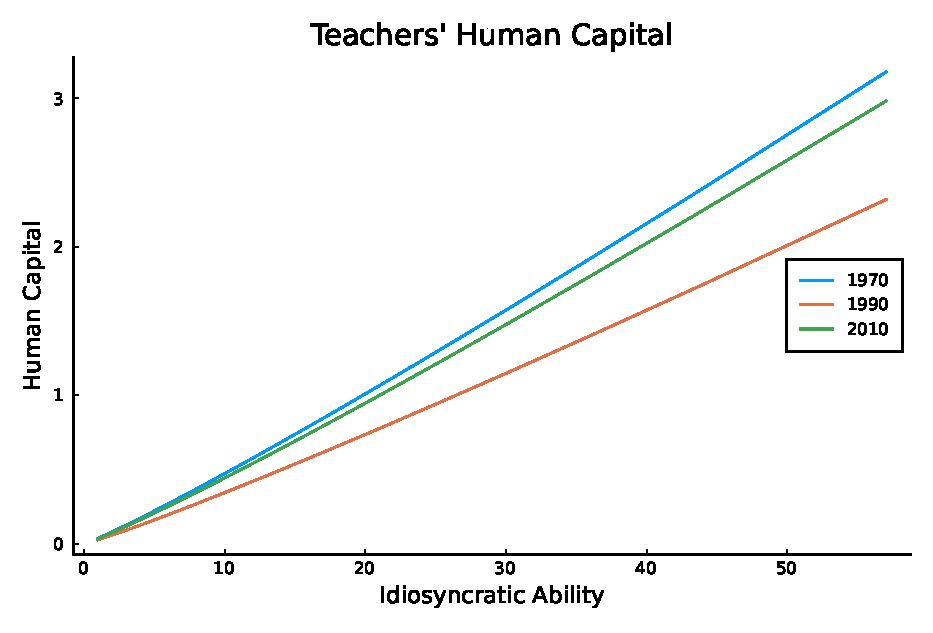
\includegraphics[width=\textwidth]{hT_men_steadystate.eps}
			% 			%\caption{ }
			% 			\label{ }
			% 		\end{center}
		% 	\end{figure}
	% \end{frame}

%\begin{frame}
%\begin{figure}
%\begin{center}
%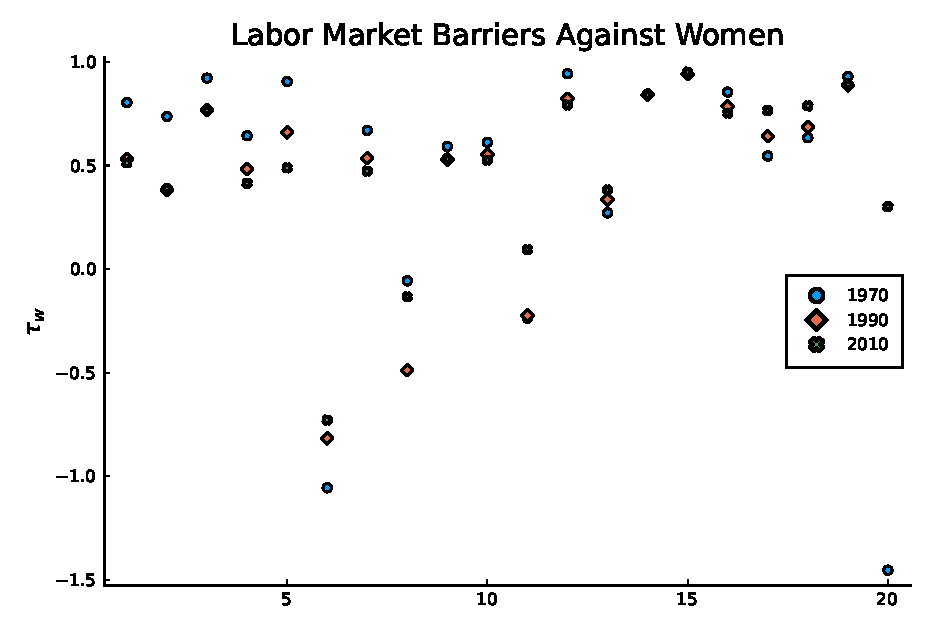
\includegraphics[width=\textwidth]{tau_w_women.eps}
%\caption{ }
%\label{ }
%\end{center}
%\end{figure}
%\end{frame}

\begin{frame}
	\frametitle{Summing up}
	
	\begin{itemize}
		\item Ability composition of teachers change over time:
		\begin{itemize}
			\item[$\circ$] Women with lower ability select into teaching career % because other careers are more attractive
			\item[$\circ$] Men with higher ability select into teaching career % because other careers are more attractive
		\end{itemize}
		\item Human capital investment drop over time, given ability % because lower ability and lower wages
		%\item $\Rightarrow$ Lower average teaching human capital 
		%\item More women become teachers
		%\item Fewer men become teachers
		%\item Smaller class sizes
		%\item $\Rightarrow$ Same level of aggregate teaching human capital 
		%\item $\Rightarrow$ Lower output 
	\end{itemize}
\end{frame}

\begin{frame}
	\frametitle{Conclusion}
	%\framesubtitle{}
	\textcolor{tblue}{Results}
	\begin{itemize}
		\item Develop a novel theory of occupational choice and human capital formation: 
		\begin{itemize}
			\item[$\circ$] non-linear wages %$\Rightarrow$ comparative and absolute advantage
			\item[$\circ$] intergenerational dynamics of human capital accumulation
		\end{itemize}
		\item Calibrate reduction in barriers
	\end{itemize}
	\textcolor{tblue}{Ongoing and Future Work}
	\begin{itemize}	
		\item Decomposition:
		\begin{itemize}
			\item[$\circ$] static gains (as in Hsieh et al., 2019) vs.
			\item[$\circ$] dynamic effects (human capital accumulation)
		\end{itemize}
		\item Multiple locations differentiated by amenities and/or local tax rates (implicit school segregation by income)
	\end{itemize}
\end{frame}

\begin{frame}
	\frametitle{Law of Motion}
	\begin{figure}
		\begin{center}
			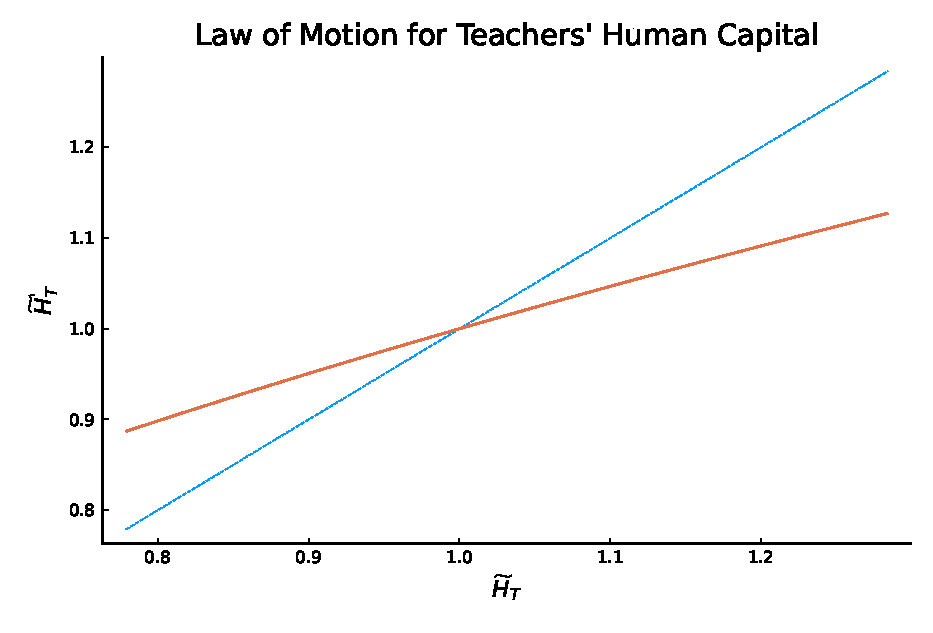
\includegraphics[width=0.8\textwidth]{plots/LoM.eps}
			%\caption{ }
			\label{ }
		\end{center}
	\end{figure}
\end{frame}

\begin{frame}
	\frametitle{Optimal Time Investment} 
	\label{timeinv}
	%The F.O.C.s for $s^T$ and $e^T$, respectively, after a few steps of algebra are:
	\begin{align}
		%\label{eq:s_T}
		s_{T,g} & = \frac{\mu \phi}{\mu \phi+\tfrac{1}{\gamma}-\eta} \nonumber\\
		%\label{eq:e_T}
		s_{O,g} & = \frac{\mu \phi}{\mu \phi+1-\eta} \nonumber
	\end{align}
	\hyperlink{eqm}{\beamergotobutton{Back}}
\end{frame}

\begin{frame}
	\frametitle{Optimal Goods Investment} 
	\label{goodinv}
	%The F.O.C.s for $s^T$ and $e^T$, respectively, after a few steps of algebra are:
	\begin{align}
		%\label{eq:s_T}
		e_{T,g} & = \left( \left(\kappa \cdot \gamma \cdot \eta \cdot \tau_{T,g} \right)^\frac{1}{\gamma} \cdot a_T^{\alpha} \cdot s_{T,g}^{\phi} \cdot \left(\tfrac{2\widetilde{H}_T}{M}\right)^{\sigma}\right)^{\frac{1}{\frac{1}{\gamma}-\eta}}  \nonumber\\
		%\label{eq:e_T}
		e_{O,g} & = \left( {{A'}_{O}} \cdot \eta \cdot\tau_{O,g} \cdot a_O^\alpha \cdot s_{O,g}^\phi \cdot  \left(\tfrac{2\widetilde{H}_T}{M}\right)^\sigma \right)^{\frac{1}{1-\eta}} \nonumber
	\end{align}
	where
	\begin{align}
		\tau_{i,g} =\frac{(1-t)(1-\tau^{\omega}_{i,g})}{1+\tau^e_{i,g}} \nonumber
	\end{align}
	\hyperlink{eqm}{\beamergotobutton{Back}}
\end{frame}

\begin{frame}
	\frametitle{Aggregate Laws of Motion} 
	\label{laws}
	\small
	%The F.O.C.s for $s^T$ and $e^T$, respectively, after a few steps of algebra are:
	\begin{align}
		%\label{eq:lomT}
		\widetilde{H}'_{T} & = \Bigg[ \left(\kappa \cdot \gamma \cdot \eta\right)^{\frac{\eta}{1-\eta\gamma}} \cdot \left(\tfrac{2\widetilde{H}_T}{M}\right)^{\frac{\sigma}{1-\eta\gamma}}\nonumber\\
		& \times \sum_{g=1}^G \tau_{T,g}^\frac{\eta}{1-\eta\gamma} \cdot \int_0^\infty  s_{T,g}^\frac{\phi}{1-\eta\gamma} \cdot a^\frac{\alpha}{1-\eta\gamma}  f_{T,g}(a)da \Bigg]^\frac{\beta}{\sigma} \nonumber\\  
		%\Bigg[ \left(\tfrac{\beta}{\sigma}\right)^\eta \cdot\eta^{\frac{1}{1-\eta}} \cdot \left(\tfrac{2\widetilde{H}_T}{M}\right)^{\frac{\sigma}{1-\eta}} \nonumber\\
		%& \times \Bigg( \frac{\sum_{i=2}^I \sum_{g=1}^G {A_i'}^\frac{1}{1-\eta}\cdot\tau_{i,g}^\frac{\eta}{1-\eta} \cdot s_{i,g}^\frac{\phi}{1-\eta}\cdot \int_0^\infty a^{\frac{\alpha}{1-\eta}} f_{i,g}(a)da}{\sum_{i=2}^I \sum_{g=1}^G f_{i,g}(a)da} \Bigg)^\eta \nonumber\\
		%& \times \Bigg(\sum_{g=1}^G \tau_{T,g}^\frac{\eta\beta }{\sigma-\eta\beta } \cdot s_{T,g}^\frac{\phi\beta }{\sigma-\eta\beta } \cdot \int_0^\infty a^\frac{\alpha\beta}{\sigma-\eta\beta } f^{g,T}(a)da \Bigg)^\frac{\sigma-\eta\beta}{\beta} \Bigg]^\frac{\beta}{\sigma} \nonumber\\
		{H}'_{O} & = \left({A'}_O \cdot \eta\right)^\frac{\eta}{1-\eta} \cdot \left(\tfrac{2\widetilde{H}_T}{M}\right)^\frac{\sigma}{1-\eta} \cdot  \sum_{g=1}^G \tau_{O,g}^\frac{\eta}{1-\eta} \cdot \int_0^\infty s_{O,g}^\frac{\phi}{1-\eta} \cdot a^{\frac{\alpha}{1-\eta}} f_{O,g}(a)da \nonumber
		%\sum_{g=1}^G \left( \tau_{O,g}^\eta \cdot \eta^\eta \cdot \left(\tfrac{2\widetilde{H}_T}{M}\right)^\frac{\sigma}{1-\eta}\cdot {A'}_O^\eta \cdot s_{T,g}^\phi \right)^\frac{1}{1-\eta}\cdot \int_0^\infty a^{\frac{\alpha}{1-\eta}} f_{O,g}(a)da \nonumber
	\end{align}
	where
	\begin{align}
		\tau_{i,g} =\frac{(1-t)(1-\tau^{\omega}_{i,g})}{1+\tau^e_{i,g}} \nonumber
	\end{align}
	\hyperlink{eqm}{\beamergotobutton{Back}}
\end{frame}

\begin{frame}
	\frametitle{Occupations} 
	\label{occupations}
	\scriptsize
	\begin{enumerate}
		\item Executives, Administrative, and Managerial
		\vspace{-0.2cm}
		\item Management Related
		\vspace{-0.2cm}
		\item Architects, Engineers, Math, and Computer Science
		\vspace{-0.2cm}
		\item Natural and Social Scientists, Recreation, Religious, Arts, Athletes
		\vspace{-0.2cm}
		\item Doctors and Lawyers
		\vspace{-0.2cm}
		\item Nurses, Therapists, and Other Health Service
		\vspace{-0.2cm}
		\item Teachers, Postsecondary
		\vspace{-0.2cm}
		\item Teachers, Non-Postsecondary and Librarians
		\vspace{-0.2cm}
		\item Health and Science Technicians
		\vspace{-0.2cm}
		\item Sales, All
		\vspace{-0.2cm}
		\item Administrative Support, Clerks, Record
		\vspace{-0.2cm}
		\item Fire, Police, and Guards
		\vspace{-0.2cm}
		\item Food, Cleaning, and Personal Services and Private Household
		\vspace{-0.2cm}
		\item Farm, Related Agriculture, Logging, and Extraction
		\vspace{-0.2cm}
		\item Mechanics and Construction
		\vspace{-0.2cm}
		\item Precision Manufacturing
		\vspace{-0.2cm}
		\item Manufacturing Operators
		\vspace{-0.2cm}
		\item Fabricators, Inspectors, and Material Handlers
		\vspace{-0.2cm}
		\item Vehicle Operators
		\vspace{-0.2cm}
		\item Home Production 
	\end{enumerate}
	
	\hyperlink{barriers}{\beamergotobutton{Back}}
\end{frame}

\begin{frame}
	\frametitle{Occupational Productivity}
	\label{aggprod}
	\begin{figure}
		\begin{center}
			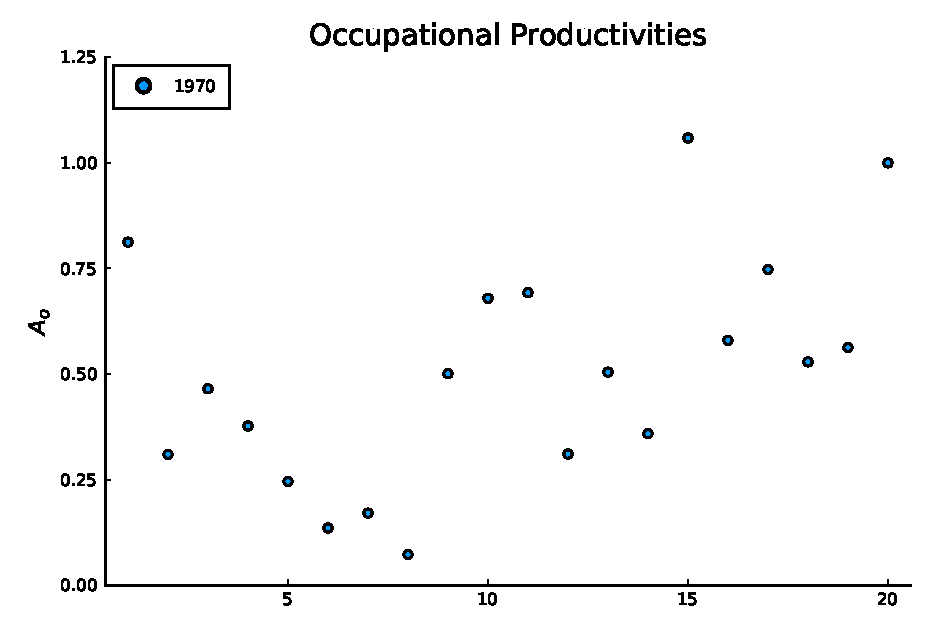
\includegraphics[width=0.8\textwidth]{plots/A_men_70.eps}
			%\caption{ }
			\label{ }
		\end{center}
	\end{figure}
\end{frame}

\begin{frame}
	\frametitle{Occupational Productivity}
	\begin{figure}
		\begin{center}
			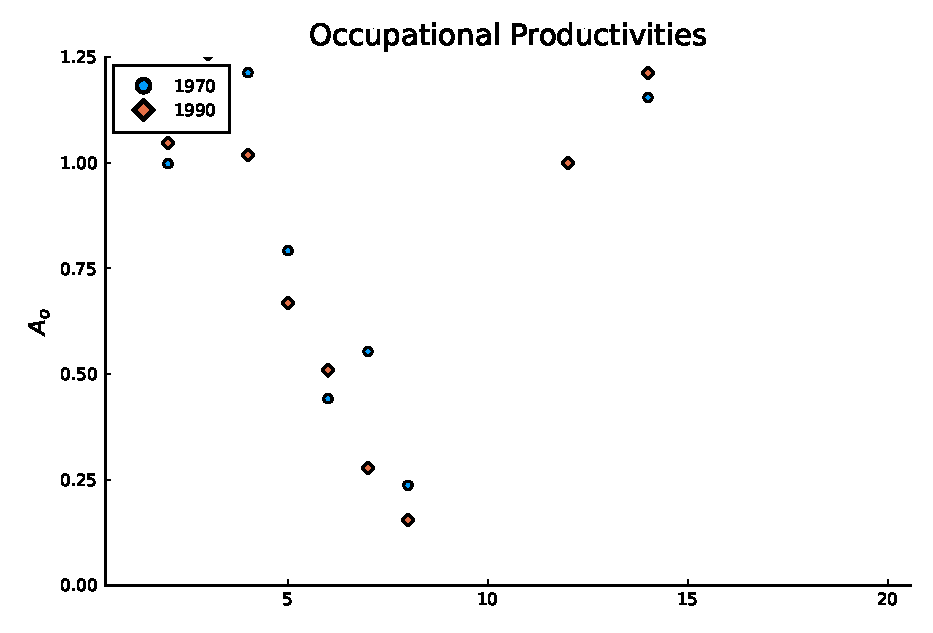
\includegraphics[width=0.8\textwidth]{plots/A_men_70_90.eps}
			%\caption{ }
			\label{ }
		\end{center}
	\end{figure}
\end{frame}

\begin{frame}
	\frametitle{Occupational Productivity}
	\begin{figure}
		\begin{center}
			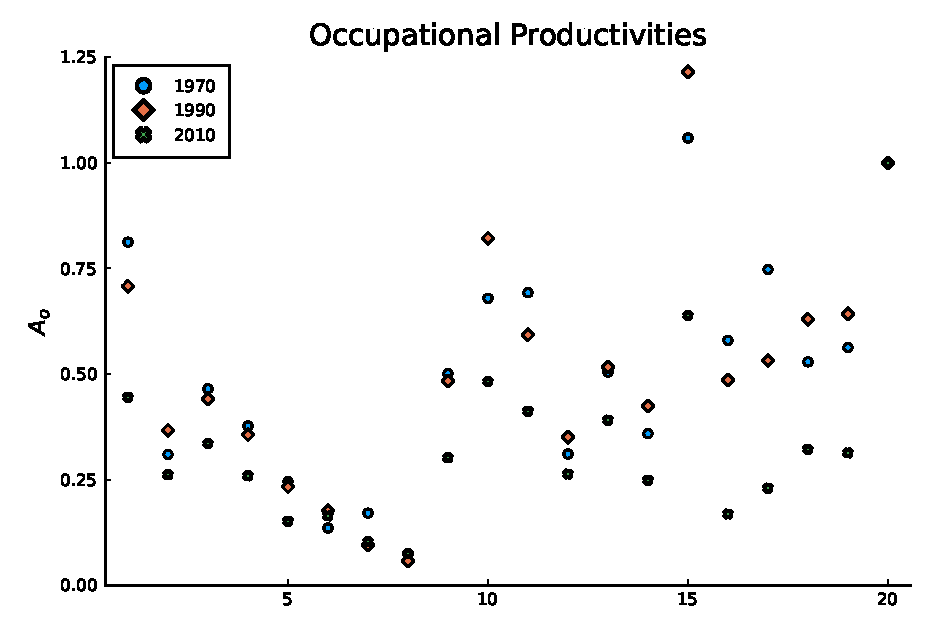
\includegraphics[width=0.8\textwidth]{plots/A_men_70_10.eps}
			%\caption{ }
			\label{ }
		\end{center}
	\end{figure}
	\hyperlink{occupations}{\beamergotobutton{Occupations}}
	\hyperlink{barriers3}{\beamergotobutton{Back}}
\end{frame}


\end{document}